% Holistic Mind final report: self-contained Overleaf / pdfLaTeX project.
% Design follows the supplied A4 article template; 11 pt matches the assessment brief.
\documentclass[11pt,a4paper]{article}
\usepackage[utf8]{inputenc}
\usepackage[T1]{fontenc}
\usepackage[english]{babel}
\usepackage{lmodern}
\usepackage{geometry}
\usepackage{setspace}
\usepackage{parskip}
\usepackage{graphicx}
\usepackage{booktabs,longtable,tabularx,array}
\usepackage{float,placeins}
\usepackage{caption}
\usepackage{amsmath,amssymb}
\usepackage{titlesec}
\usepackage{enumitem}
\usepackage{fancyhdr}
\usepackage{xcolor}
\usepackage{dashrule}
\usepackage{listings}
\usepackage[round,authoryear]{natbib}
\usepackage{xurl}
\usepackage{hyperref}
\geometry{top=2.8cm,bottom=2.5cm,left=3cm,right=3cm}
\onehalfspacing
\setlength{\parindent}{0pt}
\setlength{\parskip}{6pt}
\setlength{\emergencystretch}{2em}
\newlength{\TableInnerWidth}
\definecolor{ReportBlue}{HTML}{285D85}
\definecolor{ReportGray}{HTML}{58636D}
\hypersetup{hidelinks,hypertexnames=false,pdftitle={Holistic Mind: Final Project Report},pdfauthor={Samyam Shrestha},pdfsubject={CMP6200/DIG6200 Individual Honours Project}}
\titleformat{\section}{\large\bfseries}{\thesection}{0.5em}{}
\titleformat{\subsection}{\normalsize\bfseries}{\thesubsection}{0.5em}{}
\titleformat{\subsubsection}{\normalsize\bfseries}{\thesubsubsection}{0.5em}{}
\titlespacing*{\section}{0pt}{18pt}{10pt}
\titlespacing*{\subsection}{0pt}{12pt}{6pt}
\titlespacing*{\subsubsection}{0pt}{10pt}{4pt}
\setcounter{tocdepth}{2}
\setcounter{secnumdepth}{3}
\setlist[itemize]{leftmargin=1.2cm}
\setlist[enumerate]{leftmargin=1.2cm}
\captionsetup{font=small,labelfont=bf,justification=centering,skip=8pt}
\setlength{\textfloatsep}{16pt}
\setlength{\intextsep}{14pt}
\setlength{\LTpre}{10pt}
\setlength{\LTpost}{10pt}
\renewcommand{\arraystretch}{1.2}
\lstset{basicstyle=\small\ttfamily,breaklines=true,frame=single,rulecolor=\color{ReportGray!45},backgroundcolor=\color{ReportBlue!3},captionpos=b,columns=fullflexible,keepspaces=true,showstringspaces=false,aboveskip=10pt,belowskip=10pt}
\renewcommand{\bibsection}{\section*{References}}
\setlength{\bibhang}{1.2em}
\setlength{\bibsep}{7pt}
\pagestyle{fancy}
\fancyhf{}
\fancyhead[L]{\small Holistic Mind}
\fancyhead[R]{\small CMP6200/DIG6200 Final Report}
\fancyfoot[C]{\thepage}
\setlength{\headheight}{14pt}
\fancypagestyle{plain}{\fancyhf{}\fancyfoot[C]{\thepage}\renewcommand{\headrulewidth}{0pt}}

\begin{document}
\begin{titlepage}
\thispagestyle{empty}
\noindent\begin{minipage}[t]{0.48\textwidth}
\vspace{0pt}{\small\color{ReportGray}2025--2026 Final Project Report}
\end{minipage}\hfill
\begin{minipage}[t]{0.48\textwidth}
\vspace{0pt}\raggedleft
\IfFileExists{figures/bcu-logo.png}{\includegraphics[width=4.2cm]{figures/bcu-logo.png}}{\textbf{Birmingham City University}\\{\small Sunway College Kathmandu}}
\end{minipage}
\vspace{1.4cm}
\noindent\hdashrule{\textwidth}{0.5pt}{7pt 7pt}
\vspace{1.2cm}
\begin{center}
\sffamily
{\fontsize{14}{18}\selectfont\bfseries CMP6200/DIG6200\par}
\vspace{0.5cm}
{\fontsize{17}{22}\selectfont\bfseries Individual Honours Project (FYP)\par}
\vspace{0.6cm}
{\fontsize{18}{23}\selectfont\bfseries Final Project Report\par}
\vspace{0.8cm}
{\fontsize{22}{28}\selectfont\bfseries Holistic Mind\par}
\vspace{0.35cm}
{\fontsize{14}{20}\selectfont A Trauma-Informed Mobile Wellness Application with Explainable Hybrid Recommendations and Encrypted Journaling\par}
\end{center}
\vspace{1.2cm}
\noindent\hdashrule{\textwidth}{0.5pt}{7pt 7pt}
\vspace{1.1cm}
\noindent\begin{tabularx}{\textwidth}{@{}>{\bfseries}p{3.5cm}X@{}}
Student Name: & Samyam Shrestha \\[0.28cm]
Student ID: & 23189645 \\[0.28cm]
Programme: & BSc (Hons) Computer and Data Science \\[0.28cm]
Module: & Individual Honours Project \\[0.28cm]
Supervisor: & Rabin Ghimire \\[0.28cm]
Report Prepared: & 3 October 2026 \\
\end{tabularx}
\vfill
\end{titlepage}

\pagenumbering{roman}
\section*{Abstract}\addcontentsline{toc}{section}{Abstract}

Holistic Mind is a mobile wellness application that combines daily check-ins, personalised practice recommendations, reflective journaling, and structured learning content. Originally proposed as trauma-informed support between professional appointments for adults experiencing anxiety, ADHD, or trauma-related difficulties, the application retains a voluntary, non-diagnostic wellness scope. The project investigates how a small, explainable recommendation system can support a daily self-care routine while respecting explicitly declared comfort preferences and keeping journal content private. The artefact consists of an Expo React Native application, a Node.js and Express API, PostgreSQL, an administration dashboard, object storage, and a Python recommendation service. Its hybrid engine combines suitability rules, MiniLM semantic similarity, and, when sufficient interactions exist, collaborative evidence. Journal entries are encrypted on the device and are excluded from server-side recommendation inputs. A saved journal-free development benchmark covers 30 authored scenarios and a fixed 14-exercise catalogue. The hybrid approach achieved Precision@4 of 77.50\% and NDCG@4 of 0.7387, compared with 73.33\% and 0.7244 for rules with eligibility filtering. However, hybrid recommendations also included 3.33\% negative-labelled selections, showing that ranking improvements do not establish universal suitability. A separate eight-scenario comfort suite recorded no explicit exclusion violations. Documented simulator and backend checks support functional feasibility, while independent label review, physical-device testing, user acceptance research, and clinical effectiveness remain unverified. The contribution is an integrated, privacy-conscious software artefact with transparent evaluation and identifiable limitations.

\clearpage
{\small\setstretch{1.05}\setlength{\parskip}{0pt}\tableofcontents}
\clearpage
{\small\setstretch{1.10}\listoffigures\listoftables}
\clearpage
\pagenumbering{arabic}
\clearpage\section{Introduction}\label{sec:chapter-1}

\subsection{Background and motivation}

A daily self-care routine involves several different activities: noticing a present feeling, choosing something manageable, completing that activity, and reflecting afterwards. When these activities are disconnected, the user must repeatedly decide where to begin. Holistic Mind brings them into one mobile environment. Its intended experience is a short, voluntary sequence of check-in, practice, feedback, and reflection, supported by an exercise catalogue and a separate learning library. This project treats that sequence as a software design problem. It does not assume that using an application produces a measurable improvement in mental health.

The original proposal focuses on adults seeking support with trauma-related difficulties, anxiety, and ADHD between professional appointments \citep{shrestha2026a}. The project is motivated by the difficulty of selecting relevant content from a general library. Someone seeking focus may need a different suggestion from someone reporting low energy or feeling overwhelmed. A category label alone cannot capture every distinction, while a ranking model cannot reliably interpret every personal concern. The application therefore combines structured answers with declared comfort preferences. Personalisation is designed to organise available practices and reduce selection effort, while keeping users free to browse, decline a suggestion, or report discomfort.

\subsection{Problem statement}

The central problem is to deliver a coherent daily wellness experience without making unexplained or overly confident recommendations. Three challenges shape the implementation. First, a new account has little behavioural history, creating a cold-start problem. Second, semantic relevance does not guarantee suitability: a description can match a user's state while involving a practice they wish to avoid. Third, reflective journals contain private information that should not automatically become recommendation data. Addressing these challenges requires coordinated interface, API, ranking, storage, and evaluation decisions rather than an isolated algorithm.

\subsection{Research questions}

RQ1 asks whether a hybrid of structured suitability rules and semantic matching improves top-four recommendation relevance over random, semantic-only, and rules-based alternatives on the project's authored scenarios. RQ2 asks whether explicitly declared comfort restrictions remain enforced throughout filtering, ranking, and fallback behaviour. RQ3 asks whether persistent reflective journaling can coexist with personalisation when journal decryption remains on the user's device. These questions are deliberately bounded: the first concerns offline ranking quality, the second concerns software policy enforcement, and the third concerns an implemented privacy boundary.

\subsection{Contribution and report structure}

The contribution is an integrated mobile artefact supported by reproducible evaluation files and documented development checks. It connects account management, onboarding, daily check-ins, recommendations, practice media, feedback, encrypted journals, and managed learning content. The dissertation integrates the original proposal, interim reports, and final progress review with the current implementation and saved evaluation evidence. Section 2 reviews relevant technical ideas; Section 3 defines objectives and scope; Sections 4 to 6 explain methodology, design, and implementation; Section 7 examines testing evidence; and Section 8 evaluates the contribution and future work.

\begin{figure}[htbp]
\centering
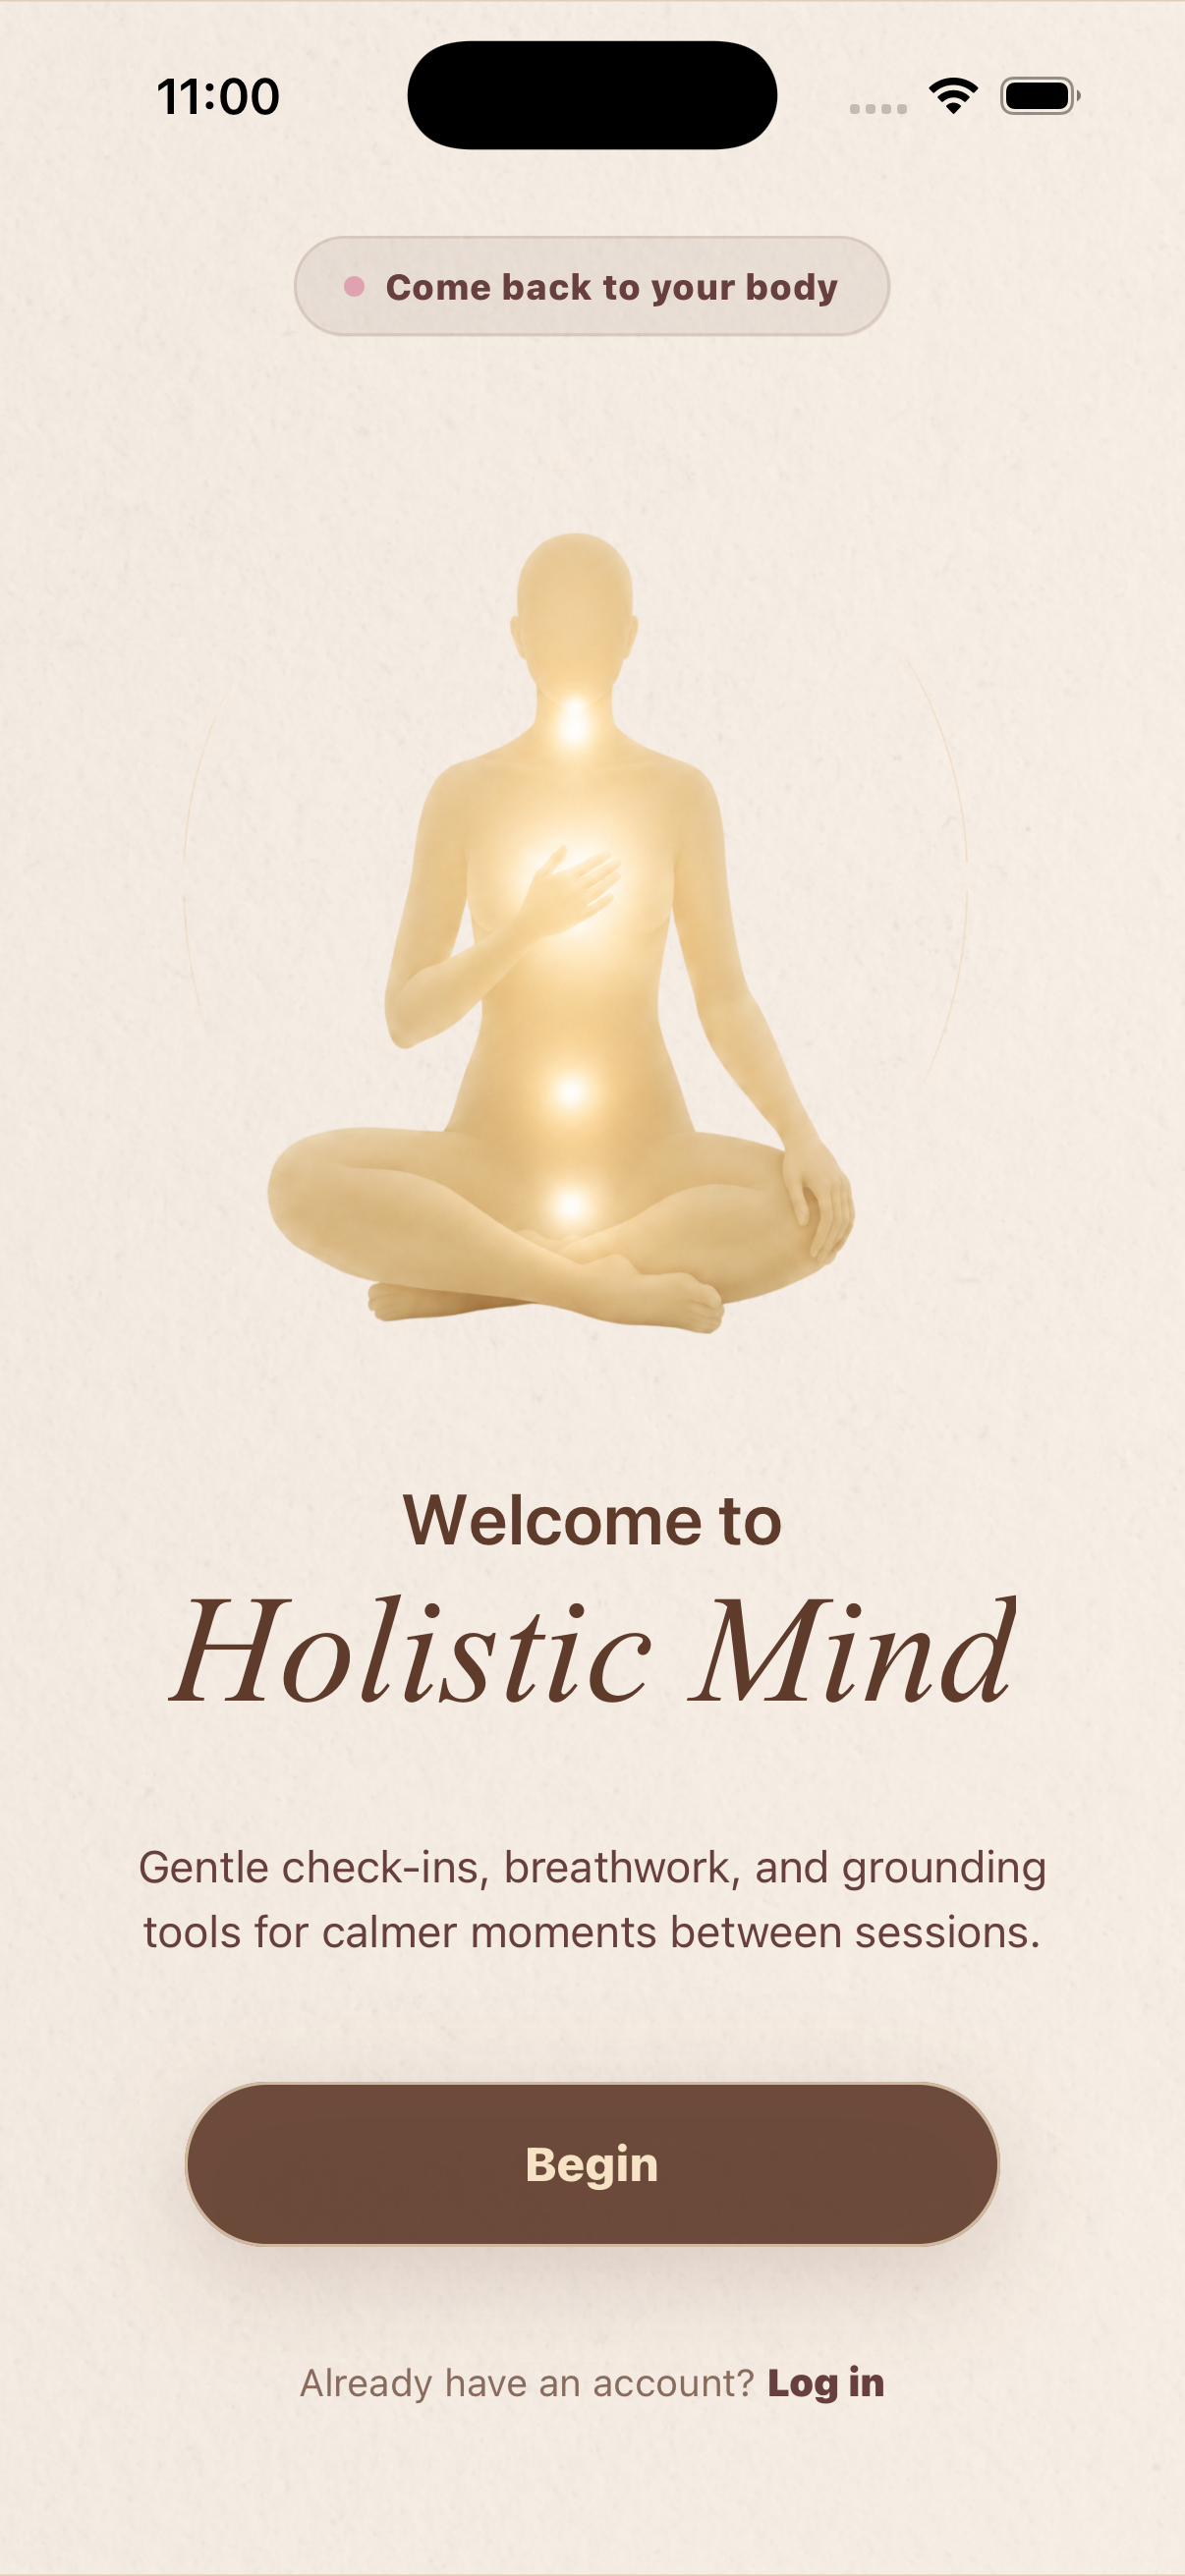
\includegraphics[width=\linewidth,height=0.62\textheight,keepaspectratio]{figures/welcome.png}
\caption[Welcome screen]{Existing iOS simulator welcome screen, captured 3 October 2026. The image illustrates the application's visual identity; it is not a usability-test result.}
\label{fig:welcome}
\end{figure}
\FloatBarrier

\subsection{Original motivation and intended users}

The proposal defined Holistic Mind as a trauma-informed mobile application for adults seeking support with childhood-trauma-related difficulties, anxiety, and ADHD between therapy sessions \citep{shrestha2026a}. That intended audience remains central to the project's design rationale. The application offers a private place to notice a current state, access a short practice, and reflect afterwards. The term trauma-informed describes an intention to respect choice, predictability, and personal comfort. It does not identify the software as a validated trauma treatment, and the application does not determine whether a user has trauma or ADHD.

The most useful element of the original proposal is its emphasis on the period between professional appointments. In that setting, a person may already have strategies they prefer but find it difficult to choose or remember one in a stressful moment. Holistic Mind organises a curated collection rather than expecting the person to search an unstructured information source. Its recommendations remain optional. A user can browse independently, avoid a particular type of practice, and provide feedback about an experience. This design addresses a concrete interaction problem while preserving the original supportive purpose.

The early proposal included a freemium commercial model and Firebase authentication. Later scope documentation placed subscription infrastructure outside the core academic deliverable. These changes distinguish the idea's commercial possibilities from what the final artefact actually implements. Likewise, the proposal's content counts describe intended delivery targets, not an audited inventory of the current catalogue. The benchmark's 14 exercises are evaluation fixtures, while the mobile application can display a larger managed catalogue. The report therefore avoids treating these different counts as interchangeable measures of completion.

\subsection{Project evolution across previous submissions}

The supplied reports form a useful sequence of decisions. The April interim report introduced a Design Science Research approach and a planned mixed-method study. The June progress review documented React Native selection, Firebase setup, initial authentication, and onboarding. Its supervisor questions asked whether a rule-based first version, explanation text, and comparison against random suggestions would be appropriate. The September final progress review then described a broader platform with custom authentication, PostgreSQL, a separate Python service, administration tools, and cloud-hosted content \citep{shrestha2026b,shrestha2026c,shrestha2026d}.

Current implementation extends that sequence with explicit comfort preferences and device-only journal encryption. The original ethical intention was that journals should not be analysed for modelling. An intermediate implementation used limited journal context, as the September review acknowledged. The present recommendation route restores a stronger separation by sending no journal text at all. This is a substantive change to the privacy and personalisation design, not merely a change in terminology. It also requires the journal-free benchmark rather than the earlier journal-containing results to represent current application inputs.

A final dissertation should explain this evolution instead of flattening every earlier statement into a claim about the final system. Firebase remains part of the documented prototype history. The September review's claim of a deployed beta describes that reported stage, while the later encrypted journal changes were verified locally and have a separate rollout status. The proposed five-participant study remains a planned activity unless participant records and analysis are supplied. These distinctions allow the original ambitions to remain visible without overstating their completion.

\clearpage\section{Review of Existing Knowledge}\label{sec:chapter-2}

\subsection{Content-based and collaborative recommendation}

Content-based recommendation matches descriptions of items to a representation of a user's interests or current context. For Holistic Mind, exercise descriptions, categories, intended states, and support goals provide this content. The approach can produce suggestions before an account has accumulated interaction history. Its weakness is dependence on the quality of metadata and the chosen similarity representation. Missing restrictions or ambiguous wording remain problematic even when a numerical similarity score is high.

Collaborative recommendation uses patterns in interaction data to estimate which items may suit a user. Holistic Mind includes a neighbour-based component, but enables it only when sufficient overlapping interactions and neighbours exist. This is appropriate because sparse histories cannot support a dependable comparison. Completion, repetition, saving, and explicit helpfulness feedback also represent different behaviours. Treating every event as equally positive would hide those distinctions. The implementation consequently assigns different values to events and prioritises uncomfortable feedback as a negative signal.

\subsection{Hybrid approaches}

\citet{burke2002} surveys ways to combine recommendation techniques and explains why hybrid systems can address weaknesses of individual methods. Holistic Mind applies that principle through eligibility filtering followed by weighted rules, semantic relevance, and conditional collaborative scoring. The rationale is complementary evidence: structured rules support predictable alignment, embeddings capture descriptive similarity, and interactions may support later adaptation. This rationale does not prove that any particular weighting is optimal; weight selection remains a separate empirical problem.

A key distinction is between eligibility and ranking. Eligibility decides whether an exercise may appear at all under the application's known restrictions. Ranking orders the remaining candidates. If restrictions were only soft penalties, sufficiently strong similarity could override them. The implemented hard exclusions avoid that failure for declared concerns. Nevertheless, they cannot address a restriction that was never collected or encoded in metadata. The system therefore needs both transparent data collection and conservative interpretation of its output.

\subsection{Semantic representations}

\citet{reimers2019} describe Sentence-BERT representations that support efficient comparison of sentences using cosine similarity. Holistic Mind uses the pretrained all-MiniLM-L6-v2 model through ONNX inference. Its model card describes a 384-dimensional representation suited to sentence and short-paragraph tasks \citep{minilm}. This supports a practical comparison between check-in descriptions and exercise documents without requiring a generative model to compose advice. The project does not fine-tune MiniLM or claim a newly trained language model.

Semantic similarity remains narrower than understanding a person's needs. A vector representation may associate related words without distinguishing whether an activity is welcome, uncomfortable, or medically inappropriate. The current engine consequently limits semantic scoring to eligible candidates and combines it with rules. Model failure is also observable: the service can identify a lexical fallback backend, while strict ONNX evaluation aborts rather than silently producing results labelled as semantic inference. This distinction makes benchmark interpretation more defensible.

\subsection{Privacy and evaluation gaps}

\citet{morris2023} demonstrate that text can be recovered from embeddings under studied attack conditions. Their work challenges the assumption that converting a journal to a vector makes its meaning private. Holistic Mind therefore uploads neither journal text nor device-generated journal embeddings for personalisation. This is a specific application design decision, not a claim that every embedding system has identical leakage. It also creates an explicit trade-off: the recommender has less reflective context available.

The reference dissertations provide useful examples of connecting architecture, implementation evidence, metrics, and critical evaluation. Rai's travel recommender and Fullel's Nepali voice assistant address different domains, datasets, and users. Their performance figures cannot validate Holistic Mind. The gap addressed here is the combination of a daily wellness workflow, declared comfort controls, and a journal privacy boundary within a small recommendation application. Clinical effectiveness, longitudinal engagement, and representative usability remain future research questions rather than established contributions.

\subsection{Implications for this project}

The reviewed ideas suggest three practical design principles. Context should be represented in a form the system can inspect, restrictions should be applied before relevance scoring, and evaluation should measure several competing outcomes. Holistic Mind uses short structured questions to make the first principle concrete, shared comfort mapping for the second, and separate quality, fill, and violation measures for the third. Together, these choices make failures easier to locate than a single opaque model output would permit.

There is also a clear gap between recommendation research and this application's eventual use. General-purpose semantic models are trained for broad language similarity rather than this exercise catalogue. Authored relevance judgments may reward descriptions that match familiar language without establishing personal usefulness. The project therefore needs domain-specific review and user-centred evidence before moving from technical feasibility to stronger effectiveness claims. This gap motivates the critical evaluation rather than undermining the value of building and testing a bounded prototype.

\subsection{Trauma-informed principles as design requirements}

SAMHSA describes trauma-informed approaches through principles including safety, transparency, peer support, collaboration, empowerment and choice, and attention to cultural and historical context \citep{samhsa}. These principles originate in wider organisational practice. Applying them to a mobile interface is an engineering interpretation that requires evaluation with its intended users. Holistic Mind chiefly operationalises choice, transparency, and predictable interaction; it does not implement every part of a comprehensive trauma-informed service.

Choice appears in optional practice selection and explicit comfort preferences. Predictability appears in short onboarding, visible navigation, and recognisable controls. Transparency appears in recommendation reasons and the explanation that journal recovery requires a separate key. The design avoids requiring a trauma narrative as the price of receiving a suggestion. Personalisation uses structured self-reports rather than an attempt to classify a person's history. The relevant question is whether these choices feel useful and respectful in practice, which cannot be answered by a software test alone.

Peer support is a clear example of a principle outside the present application. There is no evidenced moderated peer community or therapist relationship inside Holistic Mind. Cultural responsiveness is also incomplete: accepting Nepali text in an encrypted journal demonstrates text handling, not a fully localised or culturally validated intervention. Treating partial implementation honestly makes the term trauma-informed more precise. It identifies a design direction and review framework rather than certifying the application's overall suitability.

\subsection{Digital mental health evidence and its limits}

\citet{linardon2019} reviewed 66 randomised trials of app-supported smartphone interventions. Their findings support the potential of some interventions for several mental health outcomes, while noting variable trial quality and limited evidence for some outcomes. The review does not establish that Holistic Mind's specific content, recommendation rules, or intended audience will benefit. It also does not substantiate the earlier report's claim that fewer than 3\% of apps use trauma frameworks. That percentage is consequently excluded from the final argument.

The distinction matters because a functioning application and an effective intervention are different achievements. Authentication, persistent journaling, and a reliable media player can be evaluated through technical and usability methods. Claims about symptom improvement require an appropriate study design and outcome measures. Holistic Mind's evaluation is presently concentrated on software functionality and relevance agreement with authored labels. The literature motivates further research, but its findings are not transferred as outcomes of this artefact.

\subsection{Related recommender platforms and corrected sources}

The earlier interim report identified work on recommending mental health applications. Its linked 2024 paper is authored by Tapuria and colleagues, rather than the author attribution used in that draft. \citet{tapuria2024} describe requirements assessment, prototype development, and bench testing for a platform that recommends trusted mental health apps. Their emphasis on safety, confidentiality, and reliability is relevant to Holistic Mind, although recommending complete apps differs from ranking practices within one catalogue.

This comparison reinforces the importance of content quality and user requirements before algorithm complexity. Holistic Mind uses administered exercise metadata rather than choosing from independently assessed third-party applications. The administrator's publication decision therefore becomes part of the recommendation environment. Similarity scores cannot compensate for missing restrictions or unsupported descriptions. The project needs a content-review procedure alongside ranking evaluation, especially when the catalogue expands or descriptions change.

The NarraGive evaluation offers another relevant comparison. It examines content-based and collaborative recommendation of mental health recovery narratives, using measures including accuracy, precision, diversity, coverage, and unfairness \citep{slade2024}. It also respects user-blocked narratives. Holistic Mind uses different content and a much smaller authored evaluation, but the shared lesson is to assess more than relevance alone. The paper's participant outcomes and dataset are not evidence about Holistic Mind.

\citet{matthews2025} provide a scoping review specifically addressing personalisation and recommendation for mental health apps. This is a stronger source description than the abbreviated title and author details in the earlier interim bibliography. It supports positioning the project within an established research topic rather than presenting personalisation as an entirely new idea. The final report uses verified source identities and avoids inheriting unverified claims of market uniqueness.
\#\# 2.9 Literature synthesis and project positioning

Four bodies of work shape the final artefact: trauma-informed principles, evidence on digital interventions, hybrid recommendation, and privacy research. Their roles differ. Trauma-informed principles guide interaction decisions. Digital intervention evidence motivates research without validating this application. Hybrid recommendation provides a practical way to combine heterogeneous evidence. Privacy research challenges the assumption that semantic representations adequately conceal personal text. Keeping these roles distinct prevents a technology choice from becoming an unsupported clinical argument.

The project is positioned as an applied software contribution. Its originality lies in assembling an explicit daily workflow, comfort-aware eligibility, inspectable ranking, managed learning content, and device-side reflection within one system. It does not claim a first-of-its-kind app, a novel neural architecture, or an exhaustive market gap. The original proposal's focus remains meaningful without asserting that no competing application addresses similar needs. The stronger academic argument is to show the implemented mechanisms, evaluate them fairly, and identify the limits of the resulting evidence.

\clearpage\section{Aims, Objectives, and Scope}\label{sec:chapter-3}

\subsection{Project aim}

Building on the original trauma-informed support aim, the aim is to design, implement, and critically evaluate a mobile application that supports voluntary self-reflection and selection of short wellness practices through an explainable recommendation workflow. The intended outcome is a functioning software artefact with persistent account-specific data, managed content, explicit restriction enforcement, and evidence that supports carefully bounded conclusions. Success therefore includes identifying unresolved failures, rather than presenting a favourable ranking score as sufficient proof of overall quality.

\subsection{Objectives and acceptance criteria}

Objective O1 is to implement authenticated accounts, onboarding, check-ins, history, and account-specific persistence. Acceptance requires server-owned identity and separation of private records between accounts. O2 is to implement recommendations combining structured rules and semantic matching, with a documented cold-start strategy and reasons for returned exercises. O3 is to enforce declared exclusions across recommendation stages and preserve short or empty results when suitable candidates are unavailable. O4 is to support encrypted journal storage, device-side decryption, and recovery-key verification without server access to journal content.

Objective O5 is to provide administrator-managed exercises, audio, courses, modules, and related media so content changes can be made independently of a mobile release. O6 is to evaluate recommendation relevance, restriction behaviour, and documented native/\allowbreak{}backend functionality. Acceptance for O6 requires clearly identifying the dataset, baseline differences, measurement boundaries, and remaining checks. These criteria permit an honest distinction between implemented features, previously recorded passes, and capabilities that still need deployment or independent validation.

\subsection{Functional and non-functional requirements}

The main functional requirements follow the user journey. A user should create or access an account, complete short onboarding, record a daily state, receive suggestions, open a practice, provide feedback, and browse content independently. Journaling must allow private writing and later retrieval after unlocking the vault. The learning library should organise courses and modules separately from short exercises. Administrators should manage publication status and media references through protected operations. Profile features support account security, reminders, and access to configured policy or support links.

Non-functional requirements concern understandable interaction, persistent data, privacy boundaries, maintainability, and recoverable failures. The interface should clearly show selected answers, loading states, and save errors. Backend validation should reject invalid input and prevent client-selected ownership. Content and ranking services should remain separable. Secure journal design must acknowledge key-loss consequences, and recommendation behaviour must remain inspectable when dependencies fail. No unmeasured response-time target or accessibility conformance level is asserted as achieved.

\subsection{Scope boundaries}

The implemented scope includes a cross-platform codebase, with documented native validation concentrated on an iOS simulator. Local services use PostgreSQL and S3-compatible object storage; deployment documentation describes cloud arrangements. The report does not establish that every described deployment path is currently operating. The recommendation benchmark uses a fixed 14-exercise catalogue and authored scenarios rather than the entire live content system. Its results therefore describe a controlled development setting.

Diagnosis, crisis intervention, clinical prescribing, therapist messaging, and clinical outcome measurement are outside the evidenced scope. The system does not infer undeclared comfort restrictions from encrypted journals. Physical Android and iPhone release testing, independent security assessment, representative user acceptance research, and journal key rotation are incomplete. These boundaries limit the claims made in later chapters and provide concrete priorities for the next development phase.

\subsection{Requirements and implementation traceability}

The requirements below connect the original supportive purpose to observable software behaviour. Priority indicates importance to the current artefact; it does not imply that a feature has passed production acceptance. The distinction between an implemented pathway and a verified release is retained throughout the report. Requirements for a study and independent review are included because they are part of evaluating the project, even though they are not user-interface features.

\begingroup
\small\setstretch{1.08}
\setlength{\tabcolsep}{4pt}
\setlength{\TableInnerWidth}{\dimexpr\linewidth-24pt\relax}
\begin{longtable}{@{}>{\raggedright\arraybackslash}p{0.200\TableInnerWidth} >{\raggedright\arraybackslash}p{0.300\TableInnerWidth} >{\raggedright\arraybackslash}p{0.260\TableInnerWidth} >{\raggedright\arraybackslash}p{0.240\TableInnerWidth}@{}}
\caption{Functional requirements and current evidence.}\label{tab:table-1}\\
\toprule
\textbf{Requirement} & \textbf{Priority} & \textbf{Implementation location} & \textbf{Evidence state} \\
\midrule\endfirsthead
\multicolumn{4}{l}{\textit{Table \thetable\ continued}}\\
\toprule
\textbf{Requirement} & \textbf{Priority} & \textbf{Implementation location} & \textbf{Evidence state} \\
\midrule\endhead
\midrule\multicolumn{4}{r}{\textit{Continued on next page}}\\\endfoot
\bottomrule\endlastfoot
FR1 Account access and isolation & Must & Auth routes and context & Source; documented API checks \\ \addlinespace[4pt]
FR2 Onboarding and daily check-in & Must & Wellness API and Home & Source; stored choices checked \\ \addlinespace[4pt]
FR3 Explained recommendations & Must & Node route and Python engine & Saved benchmark; live request record \\ \addlinespace[4pt]
FR4 Explicit comfort exclusions & Must & Shared comfort policy & Regression and comfort-suite evidence \\ \addlinespace[4pt]
FR5 Encrypted reflection and recovery & Must & Journal context and API & Native/\allowbreak{}backend checks; rollout pending \\ \addlinespace[4pt]
FR6 Browse exercises and media & Must & Explore and exercise screens & Source; historical interface evidence \\ \addlinespace[4pt]
FR7 Structured learning library & Should & Library screens and admin & Source; interface evidence \\ \addlinespace[4pt]
FR8 Content publication management & Should & Admin and content routes & Source; earlier deployment record \\ \addlinespace[4pt]
FR9 Account controls and reminders & Should & Profile and notifications & Source; release checks incomplete \\ \addlinespace[4pt]
FR10 Representative usability study & Evaluation & Proposed study protocol & No completed study supplied \\ \addlinespace[4pt]
\end{longtable}
\endgroup

Non-functional requirements are specified through behaviour that can be checked rather than generic promises. NFR1 requires ownership to be derived from the authenticated session. NFR2 requires new journal content to leave the device only as a validated encrypted envelope. NFR3 requires model and strategy identification so semantic and fallback runs are distinguishable. NFR4 requires readable controls, visible selected states, and recoverable failures. NFR5 requires content and ranking logic to remain maintainable through separate modules and versioned evaluation artefacts. Complete accessibility conformance and quantified uptime have not been measured.

\subsection{Reconciliation of original objectives}

The original project objectives included a five-state check-in, fixed breathwork and somatic content counts, a rule-based recommendation engine with preference learning, Firebase-backed access, and evaluation with at least five intended users. The final artefact preserves the purpose of these objectives while changing their implementation. A six-dimension check-in provides more structured context than a single five-state choice. The custom API and PostgreSQL replace Firebase for account and data operations. The rule-based foundation is retained within the hybrid recommendation service.

Preference learning is implemented through interaction aggregation and conditional neighbour evidence, not automatic retraining of MiniLM after each practice. The final content system supports managed exercises and curriculum resources, but the earlier numerical content targets should be audited against a dated export before being marked complete. The freemium idea has not become an evidenced payment system. These are sensible scope decisions, provided the report describes them as changes rather than treating every initial objective as achieved in its original form.

The user-study objective is the most significant incomplete research commitment. Earlier reports describe intended recruitment, SUS-based usability assessment, relevance ratings, and interviews. No participant-level data, completed questionnaires, consent records, interview analysis, or results accompany the current material. The dissertation therefore presents the study design as future evaluation and uses the authored benchmark for its actual ranking evidence. Appendix C provides a concrete protocol that can be used to close that gap without manufacturing a study outcome.

\clearpage\section{Project Design and Methodology}\label{sec:chapter-4}

\subsection{Development approach}

The project documentation records an iterative development process organised around a 15-week journal. Early stages addressed problem definition, requirements, interface planning, and navigation. Subsequent work connected onboarding, check-ins, journals, authentication, persistent storage, content administration, and recommendations. Later changes introduced stronger privacy and comfort controls. The journal is a development record rather than independently verified time-sheet evidence. It supports an account of sequencing, but does not establish the exact effort spent on each activity.

Iterative delivery suits this artefact because changes in one component expose requirements in another. For example, device-only journal encryption changes both the journal API contract and the recommender's available inputs. Comfort preferences require corresponding metadata, backend mapping, fallback handling, and tests. Small vertical increments help expose these dependencies before the system is treated as complete. However, iteration can also leave older documentation inconsistent with newer source, so the report prioritises current routes and the journal-free evaluation over historical descriptions.

\begin{figure}[htbp]
\centering
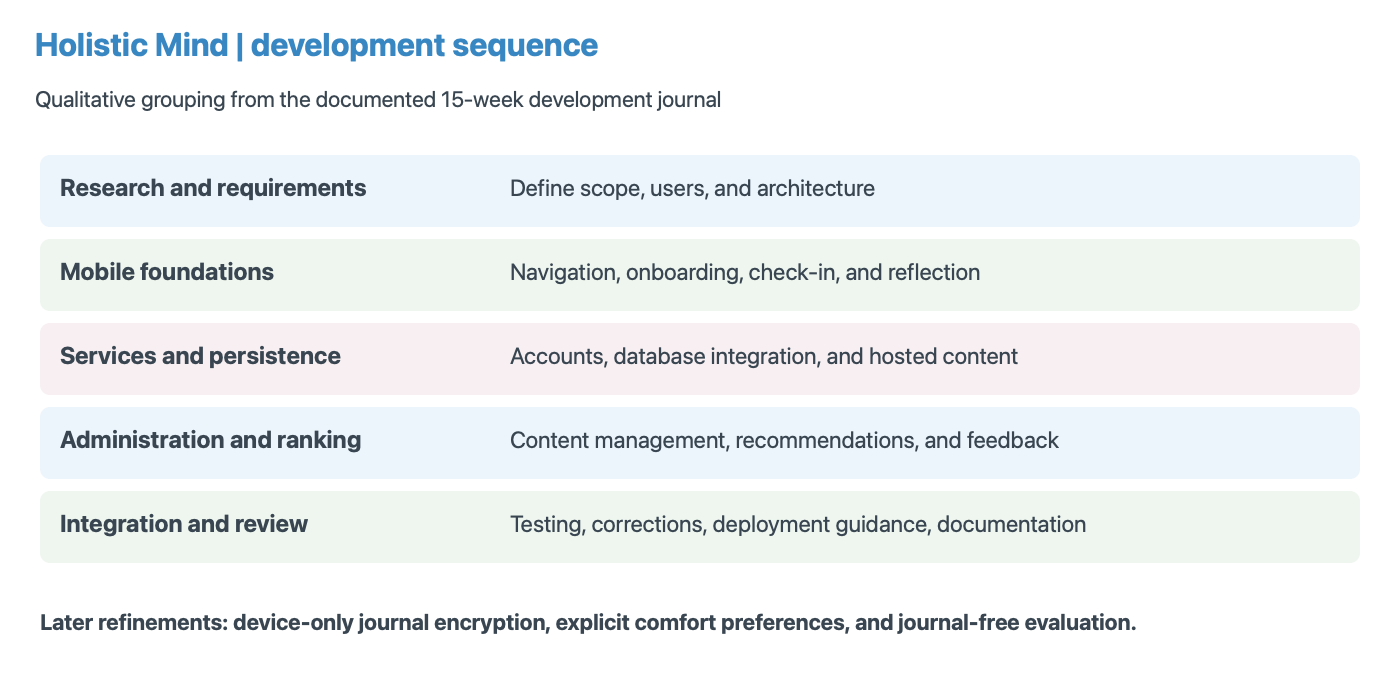
\includegraphics[width=\linewidth,height=0.62\textheight,keepaspectratio]{figures/timeline.png}
\caption[Development sequence]{Development phases summarised from the project's 15-week journal. Later privacy and evaluation refinements are shown separately; the graphic is a qualitative sequence, not measured effort.}
\label{fig:timeline}
\end{figure}
\FloatBarrier

\subsection{Technology selection}

Expo React Native and TypeScript provide a shared mobile implementation and typed integration between screens and services. Node.js with Express manages authenticated application operations, while PostgreSQL stores relational wellness and content records. A Python FastAPI service isolates numerical recommendation work from account and content APIs. ONNX inference keeps the pretrained embedding model within the recommendation service. The architecture adds operational complexity compared with a single process, but gives each component a clear responsibility.

Object storage holds larger media assets, avoiding their inclusion in ordinary database rows or every application bundle. A separate React administration interface allows structured content updates. These decisions are appropriate to the existing codebase and content requirements; they are not the result of a formal comparison of every available framework. Maintaining several runtimes, schema migrations, native builds, and storage policies remains a cost that must be considered alongside flexibility.

\subsection{Evidence and evaluation strategy}

The evaluation uses several evidence types because no single test answers all objectives. Offline ranking files compare recommendation approaches. Restriction tests exercise explicit exclusions and insufficient candidate pools. Journal cryptography and API tests address envelope validation, ownership, and migration. The device-and-backend record describes previous checks against a simulator and running development services. Source inspection establishes what is implemented, but it cannot demonstrate that a production deployment behaves identically.

The main ranking dataset contains 30 authored personas, each with relevance labels for all 14 benchmark exercises. Labels range from negative suitability to strongest relevance. The production suite removes synthetic journal inputs while retaining the original scenario labels. Ten repetitions per persona support timing measurement and random-baseline variation. They do not create 300 independent people. A separate eight-scenario suite examines declared comfort restrictions. The suites are reported separately because their purposes and input distributions differ.

\subsection{Ethical and methodological controls}

The report uses supplied dissertations as structural references without adopting their instructions, declarations, participant claims, or results. Existing project screenshots illustrate interfaces, while architectural figures explain source-observed behaviour. Reported benchmark values come from saved project artefacts. No new participant study is invented, and documented development passes are attributed to their original test record. This separation makes it possible to assess implementation without implying evidence that does not exist.

Privacy is considered throughout the architecture rather than added only to the discussion. Journal encryption reduces server access to reflective content, while structured check-ins and interaction data remain server-readable. The distinction should be explained to users. Synthetic scenarios reduce the need to expose real journals during development, but cannot replace independent expertise or diverse real-world experience. Any later user study should define consent, withdrawal, data minimisation, and a suitable research protocol before recruitment.

\subsection{Design Science Research framing}

\citet{hevner2004} describe design science as research through building and evaluating information-system artefacts. This provides the methodological foundation proposed in the April interim report. Holistic Mind instantiates that approach through an application, a recommendation mechanism, and a privacy architecture that respond to a defined problem. The research contribution is assessed through documented behaviour and evaluation, rather than the existence of code alone.

The project's problem phase identified fragmented daily support and the burden of choosing content. The construction phase developed the mobile interface and connected services. Evaluation then exposed practical issues: native dependencies missing from a build, secure-storage signing requirements, recommendation exclusions, and the impact of removing journal context. These findings prompted targeted refinements. The resulting learning is specific to the artefact: restrictions need a shared policy, privacy changes need new evaluation inputs, and native integration needs installed-build verification.

A limitation of the research process is that technical evaluation progressed further than evaluation with intended users. The artefact therefore has stronger evidence for data flow and restriction enforcement than for perceived usefulness. A mature DSR account should acknowledge that imbalance and specify what the next evaluation cycle must resolve. The report does so through a study protocol, independent content-review priorities, and a release-verification plan. This is a defensible partial research outcome rather than a claim that construction alone proves the design successful.

\subsection{User-centred design activities and boundaries}

The earlier reviews emphasised friendly onboarding and the risk of making sensitive questions clinical or overwhelming. That rationale is reflected in short options, supportive wording, and the ability to choose a support goal without describing traumatic experiences. Interface refinement also addressed spacing, card size, text wrapping, and navigation. These activities show attention to the user's interaction burden, although developer-led iteration is different from systematic observation of a representative user group.

The next user-centred cycle should test the user's understanding of the complete journey. A participant should be able to explain what a check-in contributes, distinguish a suggestion from an instruction, identify how to avoid a practice, and understand the recovery consequences of encrypted journaling. Observing these tasks would be more informative than asking only whether the screen looks attractive. It would also reveal whether privacy explanations create confusion or prevent a person from completing setup.

\subsection{Feasibility and resource constraints}

The April plan described a nine-month project, while the repository contains a fifteen-week development journal. These sources represent different planning views rather than interchangeable records of elapsed effort. The dissertation uses dated submissions to establish major milestones and the development journal to describe work phases. It does not infer an exact completion percentage from either. That avoids an apparent discrepancy being resolved through invented dates or effort estimates.

Technical feasibility rests on the existing integration of mature components: a shared mobile codebase, typed API modules, relational persistence, object storage, and a compact pretrained embedding model. Operational feasibility is more demanding because the project now contains multiple services and native dependencies. A stopped API can prevent sign-in despite correct Google configuration. A stale container can return an older ranking version despite updated source. These examples show why service readiness and version identification are practical requirements.

Content production is a separate resource constraint. Audio, video, written guidance, and curriculum structures require review and consistent metadata as well as upload tooling. The administration dashboard reduces release friction, but it does not remove that editorial workload. A staged content release is more feasible than assuming every proposed module can be produced and validated immediately. The original idea of optional later modules should remain a roadmap rather than a reason to delay validation of the core daily loop.

\subsection{Risk management and ethical feasibility}

The earlier reports identify recruitment difficulty, content delays, recommendation complexity, possible participant distress, and platform-release constraints. Their mitigation ideas remain useful, but Firebase billing risks are no longer an adequate description of the current system. Current operational risks include multi-service availability, public and private storage configuration, recovery-key loss, unsuitable metadata, and the compatibility of native builds with backend changes.

\begingroup
\small\setstretch{1.08}
\setlength{\tabcolsep}{4pt}
\setlength{\TableInnerWidth}{\dimexpr\linewidth-24pt\relax}
\begin{longtable}{@{}>{\raggedright\arraybackslash}p{0.250\TableInnerWidth} >{\raggedright\arraybackslash}p{0.290\TableInnerWidth} >{\raggedright\arraybackslash}p{0.180\TableInnerWidth} >{\raggedright\arraybackslash}p{0.280\TableInnerWidth}@{}}
\caption{Current project risk register. Ratings are qualitative planning judgments, not measured incident probabilities.}\label{tab:table-2}\\
\toprule
\textbf{Risk} & \textbf{Likelihood} & \textbf{Impact} & \textbf{Control or next action} \\
\midrule\endfirsthead
\multicolumn{4}{l}{\textit{Table \thetable\ continued}}\\
\toprule
\textbf{Risk} & \textbf{Likelihood} & \textbf{Impact} & \textbf{Control or next action} \\
\midrule\endhead
\midrule\multicolumn{4}{r}{\textit{Continued on next page}}\\\endfoot
\bottomrule\endlastfoot
Unreviewed exercise metadata & Medium & High & Independent review; version catalogue \\ \addlinespace[4pt]
Lost journal recovery material & Medium & High & Clear backup confirmation; recovery tests \\ \addlinespace[4pt]
Outdated app or container version & Medium & High & Version checks; coordinated release \\ \addlinespace[4pt]
Wrong storage access configuration & Medium & High & Separate public content from private data \\ \addlinespace[4pt]
Recruitment or ethics delay & Medium & Medium & Approve protocol before scheduling study \\ \addlinespace[4pt]
Media or content production delay & Medium & Medium & Publish reviewed core content in stages \\ \addlinespace[4pt]
Native signing or module mismatch & Medium & Medium & Test installed signed builds \\ \addlinespace[4pt]
Unclear recommendation explanation & Medium & Medium & Task-based usability assessment \\ \addlinespace[4pt]
\end{longtable}
\endgroup

Risk management should be proportionate to actual operations. Synthetic test accounts and fixtures permit technical verification without exposing real reflective histories. A future study with the intended audience requires its own consent process and support arrangements. The application should not ask participants to disclose a trauma story to qualify for a usability task. No claim of ethics approval, clinical review, or regulatory compliance is made merely because these controls appear in a plan.

\clearpage\section{Artefact Design}\label{sec:chapter-5}

\subsection{System architecture}

The mobile application communicates with the Node API, which authenticates requests and coordinates persistence, content access, and recommendation generation. The API queries PostgreSQL for account-specific context and published recommendable exercises, maps comfort choices to constraints, pseudonymises interaction identifiers, and calls the Python service. Returned items are recorded and exposed through the application. The administrator uses protected content endpoints and signed media-upload operations. Figure~\ref{fig:architecture} separates these responsibilities and shows the journal boundary alongside the ordinary application data flow.

Keeping the recommender behind the API prevents the mobile client from directly deciding another account's context. PostgreSQL provides relationships and transaction support; object storage handles media delivery separately. A signed URL grants a bounded storage operation without distributing permanent storage credentials to the client. These are design mechanisms rather than evidence of a completed security audit. Service configuration, deployment policies, and operational logging must preserve the same boundaries in a release environment.

\begin{figure}[htbp]
\centering
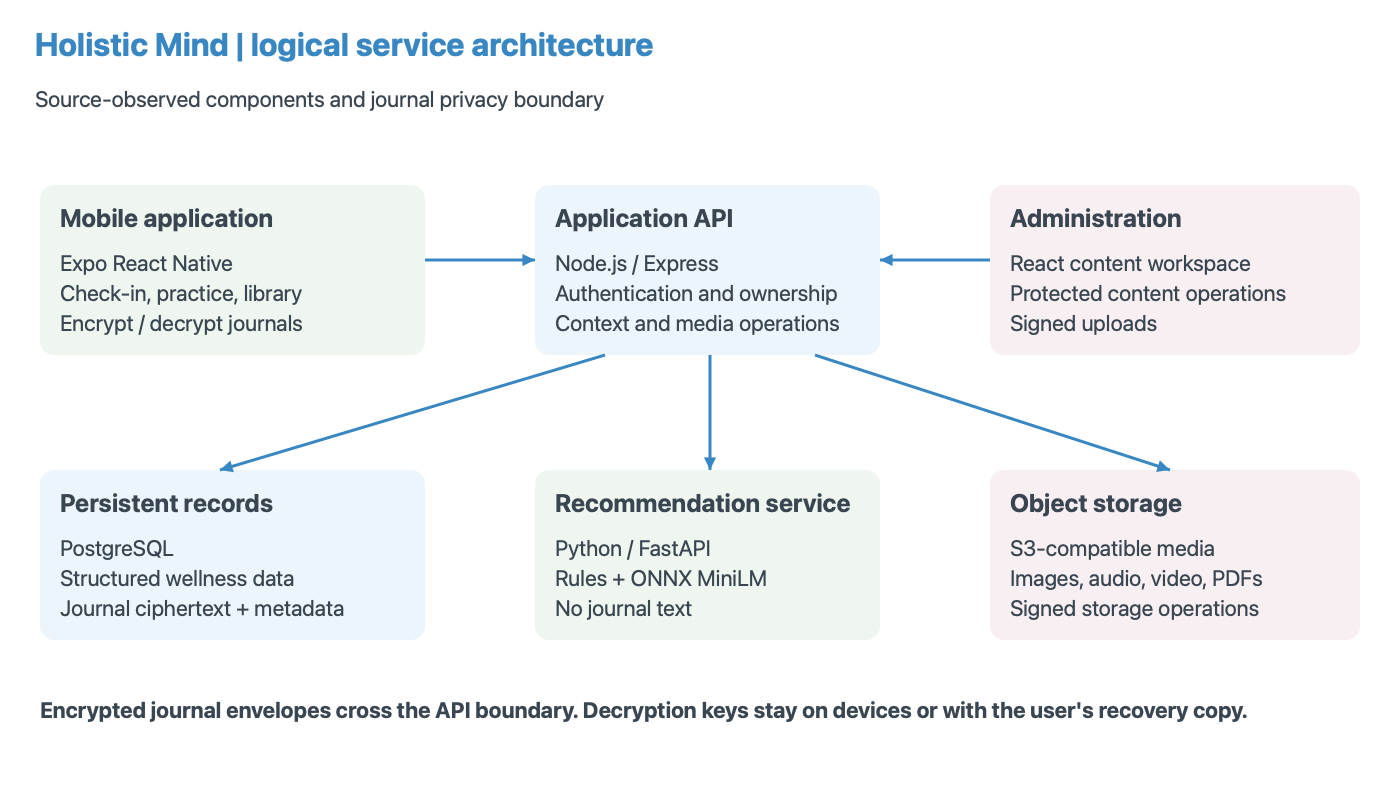
\includegraphics[width=\linewidth,height=0.62\textheight,keepaspectratio]{figures/architecture.png}
\caption[Logical service architecture]{Current logical architecture reconstructed from source. Journal content is encrypted before upload; structured wellness context reaches the separate recommendation service.}
\label{fig:architecture}
\end{figure}
\FloatBarrier

\subsection{User journey and interface design}

The user journey begins with welcome, account access, and brief onboarding. The Home screen prioritises daily check-in and relevant next actions. Explore offers user-led browsing, Journal provides reflective writing, Library organises learning content, and Profile manages account-related settings. History presents previous activity and check-in information. This arrangement gives personalisation a clear place without requiring every activity to start from a recommendation.

The visual design uses warm neutral backgrounds, rounded components, body-based illustrations, and restrained accent colours. Selected states, readable spacing, and short prompts aim to reduce interaction complexity. Figure~\ref{fig:journey} shows the daily loop, while Figure~\ref{fig:library} later illustrates the implemented library screen. These observations describe design intent. Without measured task completion, accessibility testing, or participant feedback, the report cannot conclude that the interface is easy for every target user.

\begin{figure}[htbp]
\centering
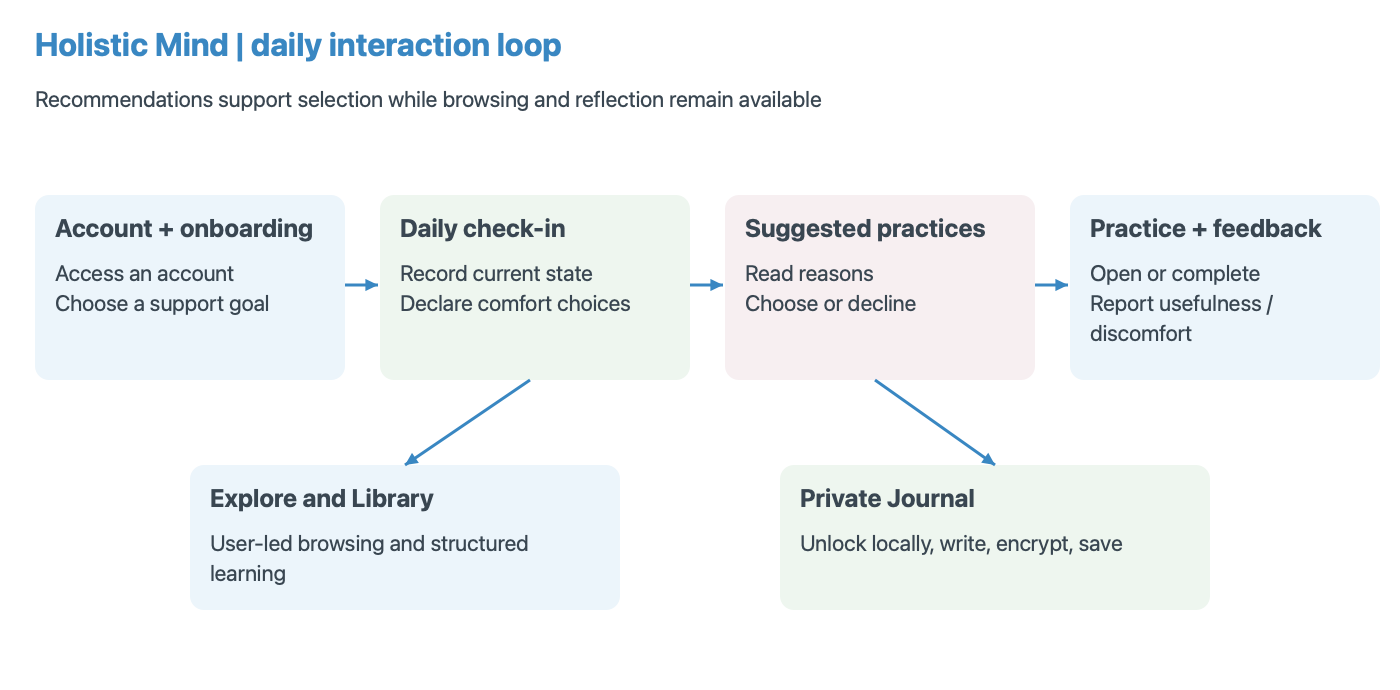
\includegraphics[width=\linewidth,height=0.62\textheight,keepaspectratio]{figures/journey.png}
\caption[Daily user journey]{Daily user journey. Browsing and encrypted reflection remain voluntary parallel paths; practice feedback contributes to later recommendations.}
\label{fig:journey}
\end{figure}
\FloatBarrier

A practical example clarifies the interaction. A user reports feeling scattered and selects focus as the immediate support need. If the same user also avoids breath holds, the recommendation pathway must remove exercises requiring that action before deciding which remaining practice best matches focus. The interface should present the resulting options as suggestions with reasons, and the user may still choose another activity through Explore. Reporting discomfort provides additional evidence for future exclusions. This example illustrates the intended sequence, not a new measured test case or a claim about the user's eventual response to a practice.

\subsection{Data model and ownership}

Private records are associated with a server-established user identity. The principal groups include accounts and profiles, authentication sessions, onboarding responses, daily check-ins, encrypted journal entries and vault records, recommendation requests and items, and interaction feedback. Content groups include exercises, media, courses, modules, and related learning resources. Figure~\ref{fig:data} presents a simplified relationship map; it deliberately omits operational columns and is not a substitute for the actual migration definitions.

Ownership matters especially when reading journals, retrieving history, or submitting recommendation feedback. Knowing an object identifier should not grant access to another account's record. Recommendation feedback is tied to an exercise returned in an owned request. The journal API validates versioned envelopes while deriving the account from authentication. These checks complement database relationships: a schema can express associations, but application queries must still apply account boundaries consistently.

\begin{figure}[htbp]
\centering
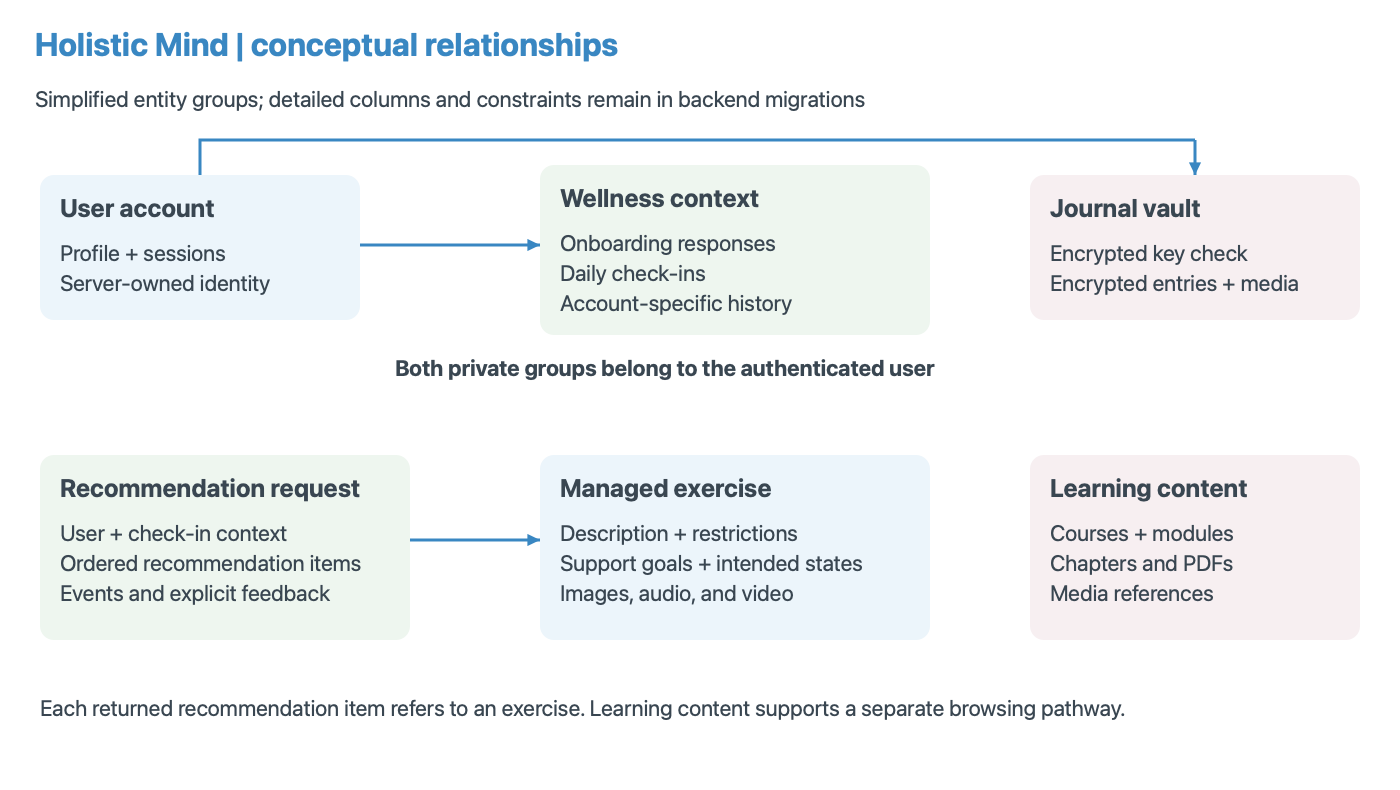
\includegraphics[width=\linewidth,height=0.62\textheight,keepaspectratio]{figures/data.png}
\caption[Conceptual data relationships]{Simplified conceptual data relationships. Private wellness records belong to users; recommendation items refer to managed exercise content.}
\label{fig:data}
\end{figure}
\FloatBarrier

\subsection{Recommendation pipeline}

The pipeline first constructs eligible candidates using known contraindications and explicit exclusions. It then builds text documents from current check-in answers, the onboarding goal, and exercise metadata. The current application sends an empty journal list. After tokenisation and ONNX inference, normalised embeddings support cosine-based comparison. Structured rules assess alignment with declared needs. Collaborative evidence is considered only when interaction overlap and neighbour thresholds are met. This sequencing prevents a filtered exercise from re-entering through a later scoring component.

In cold start, the base score is S = 0.72R + 0.23C + 0.05H, where R represents rules, C current-context similarity, and H goal/\allowbreak{}history similarity. When collaboration is active, S = 0.65R + 0.20C + 0.05H + 0.10B, with B the collaborative component. The engine subtracts recency penalties and uses category diversity during selection. Primary-support alignment and a limited fresh-item substitution may also shape the final list. Consequently, a returned position is not simply a sorted semantic score.

\begin{figure}[htbp]
\centering
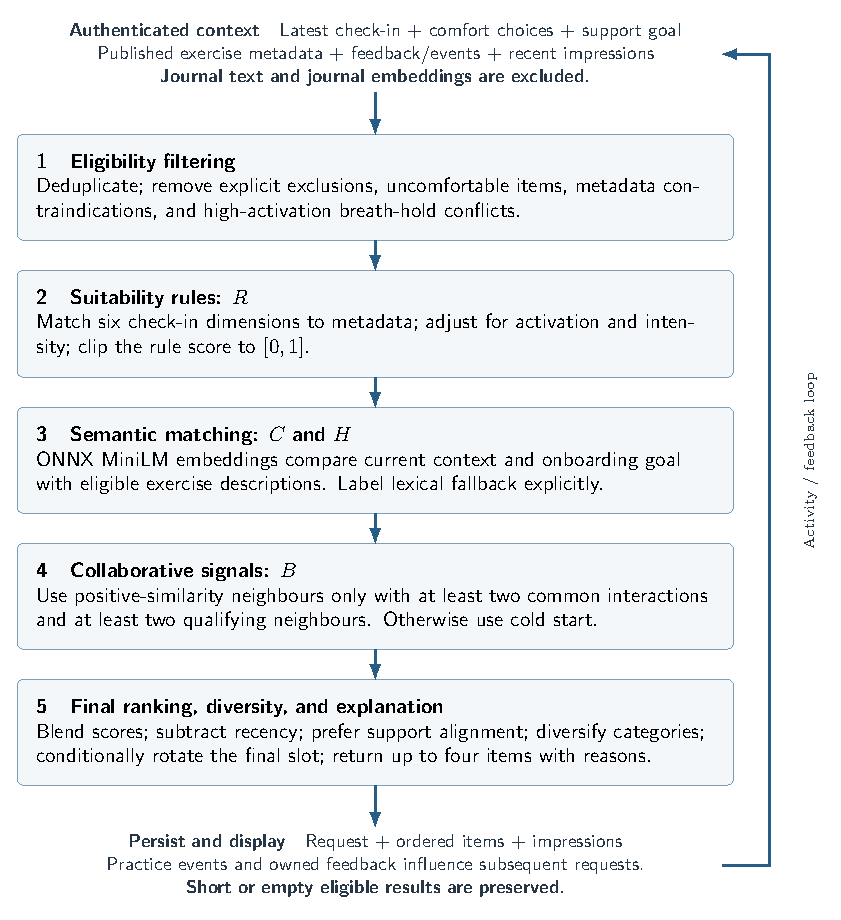
\includegraphics[width=\linewidth,height=0.70\textheight,keepaspectratio]{figures/recommendation-five-stages.pdf}
\caption[Five-stage recommendation engine and feedback loop]{The five-stage recommendation engine and feedback loop. Eligibility is enforced before any scoring; journal text and embeddings are excluded from current application requests.}
\label{fig:recommendation-five-stages}
\end{figure}
\FloatBarrier

\subsection{Privacy design}

Journal content uses a separate trust boundary from recommendations. A device generates a random 256-bit key, encrypts entry content using XChaCha20-Poly1305 with a fresh 24-byte nonce, and uploads an authenticated envelope. Associated data binds encryption to identifiers and purpose. Native key storage uses account-scoped SecureStore; web unlocks keep the key in memory. Recovery imports the user's recovery key and verifies an encrypted known value. Figure~\ref{fig:privacy} shows how persistent storage can coexist with device-side decryption.

The server can still observe ownership, timestamps, counts, identifiers, and ciphertext lengths. Check-ins, comfort choices, and feedback also remain readable to application services. Losing every device key and recovery copy makes encrypted entries unrecoverable. Ordinary account-password reset does not restore journal access. Existing plaintext entries require an explicit migration path, and clearing current database fields does not erase earlier backups. These limits are essential to describing what the privacy design actually protects.

\subsection{Relational modelling and consistency}

The database design builds on a clear separation between account identity, private activity, content, and recommendation evidence. A user row provides the ownership reference for profiles, sessions, onboarding, check-ins, journals, and recorded practice. Managed content has its own identifiers and publication lifecycle. Recommendation requests retain model version and context, while returned items preserve position, score components, reason, and exploration status. This supports a later explanation of which engine produced a displayed result.

Several source-defined constraints make application assumptions explicit. Email addresses are unique and normalised. Check-ins are unique per user and date, allowing a same-day update without creating multiple daily records. Recommendation items are unique within a request and occupy distinct positions. Feedback values have bounded helpfulness and enumerated state-change fields. Foreign-key cascades support deletion of user-linked data, but records outside the application database, such as retained exports or copied recovery keys, require separate handling.

PostgreSQL's JSONB fields accommodate variable answer and envelope structures without abandoning relational ownership. Arrays store exercise tags and goals, while constraints restrict activation and intensity values. This is a more appropriate account of flexibility than assuming every varying field requires a document database. The Modern Data Stores coursework provides a useful precedent for matching storage to workload, but Holistic Mind does not implement that coursework's MongoDB replica set or MQTT ingestion.

Indexes correspond to frequent access patterns: user-and-date lookup for check-ins, user-and-created-time retrieval for reflections and practice events, and publication-order lookup for exercises and courses. Their existence is source evidence, not a measured database-performance result. A future load test should inspect query plans and concurrency under realistic catalogue and account volumes. Small local datasets cannot establish the scaling behaviour of a deployed service.

\subsection{API contracts and sequence design}

A recommendation request is a coordinated sequence rather than a direct model call. Authentication establishes the user. The Node route loads the latest check-in and published recommendable content, derives restrictions, aggregates interactions, and prepares a pseudonymous context. The Python response identifies the model and strategy and supplies up to the requested number of items. The Node layer records the request and items, allowing subsequent events and feedback to be tied to what was actually returned. Figure~\ref{fig:sequence} summarises this sequence.

\begin{figure}[htbp]
\centering
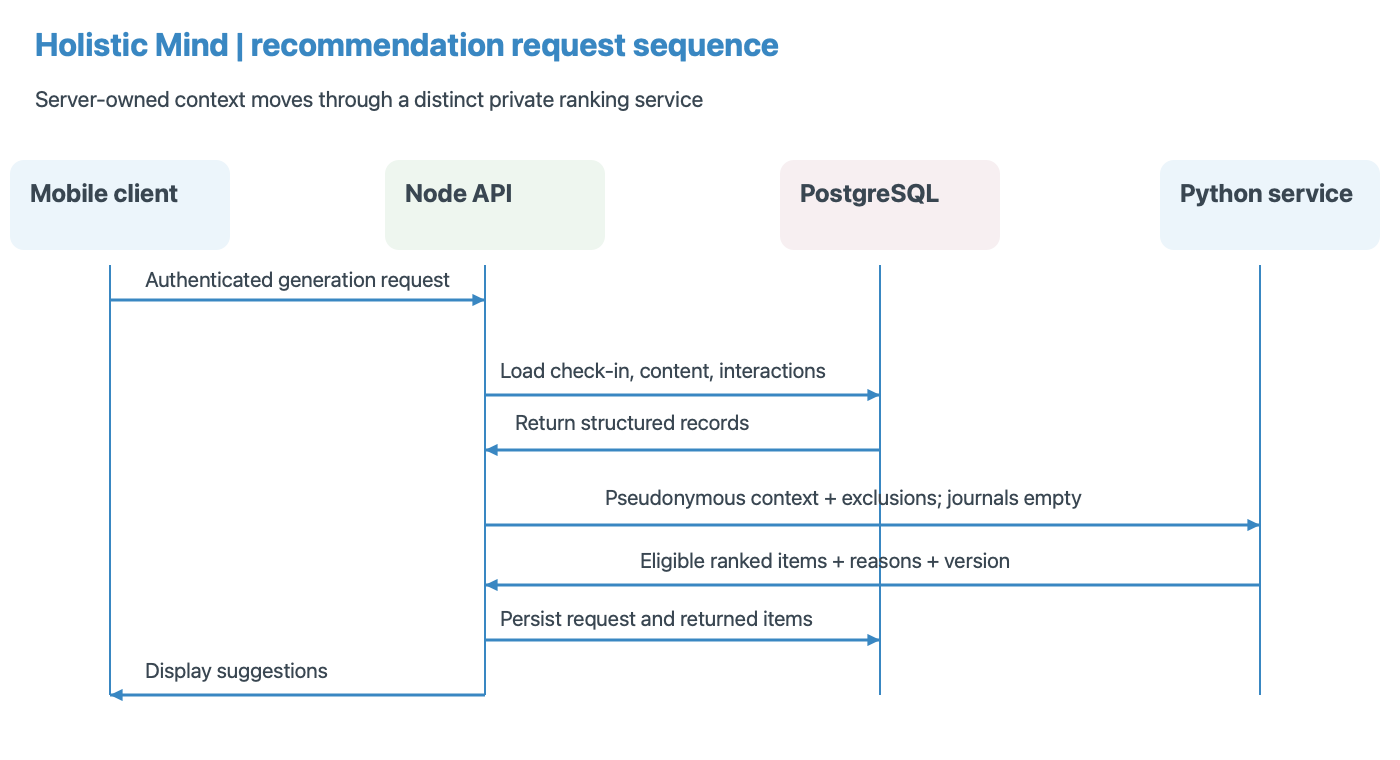
\includegraphics[width=\linewidth,height=0.62\textheight,keepaspectratio]{figures/sequence.png}
\caption[Recommendation API sequence]{Source-grounded recommendation request sequence, including authentication, contextual queries, constrained ranking, and persistence of returned items.}
\label{fig:sequence}
\end{figure}
\FloatBarrier

The contract has meaningful error states. A missing check-in prevents recommendation generation rather than permitting the client to fabricate server context. An unavailable published catalogue differs from an eligible set emptied by restrictions. A service failure may activate the application's separate fallback, while a successful empty result must remain empty. Each state has a different user-facing implication and should remain distinguishable in integration tests.

Journal operations have a different contract. Vault creation stores an encrypted check value, new entry writes accept envelopes, and normal reads return encrypted entries. A dedicated legacy path exposes older records only to the authenticated owner for migration. Media operations validate account and entry relationships. Separating these routes helps the interface explain whether it needs login, journal unlock, recovery material, or a retry of the network operation. A single generic save failure would obscure those distinctions.

\subsection{Media and publication lifecycle}

The content pipeline separates record creation from media upload and publication. An administrator requests a signed upload, transfers the asset to S3-compatible storage, and associates its reference with the appropriate record. Media and catalogue states distinguish drafts from ready or published content. The current upload helpers use a fifteen-minute expiry. A valid signed operation does not guarantee that the resulting media is correctly encoded or that its associated guidance has been reviewed, so readiness checks remain necessary.

Learning resources may be public or publicly retrievable according to deployment configuration, while encrypted journal attachments follow a different API and storage path. The existence of public educational media should not lead to treating private reflection as another content upload. The administrator's content-promotion scripts also have a different purpose from a backup of account data. These distinctions are inherited from the project's final progress review and made more explicit in the current design.

\clearpage\section{Implementation}\label{sec:chapter-6}

\subsection{Mobile application and state management}

The mobile source separates screens, services, shared types, navigation, context, and theme definitions. Authentication context manages account state, journal context coordinates unlock and entry operations, and audio-player context supports playback across screens. Service modules centralise API access rather than embedding every network request in presentation components. This structure helps changes such as a new journal envelope format propagate through a defined layer while preserving the screen's writing interaction.

The application includes dedicated authentication and account-security screens, multi-step check-in components, exercise detail and playback, free writing, prompted journaling, course navigation, and PDF viewing. Recent source also includes journal attachment composition and media handling. Their existence is implementation evidence, but the earlier documented simulator checks should not be stretched to cover every later attachment path. The report therefore treats the wider media feature set as source-observed capability requiring release-level verification.

\begin{figure}[htbp]
\centering
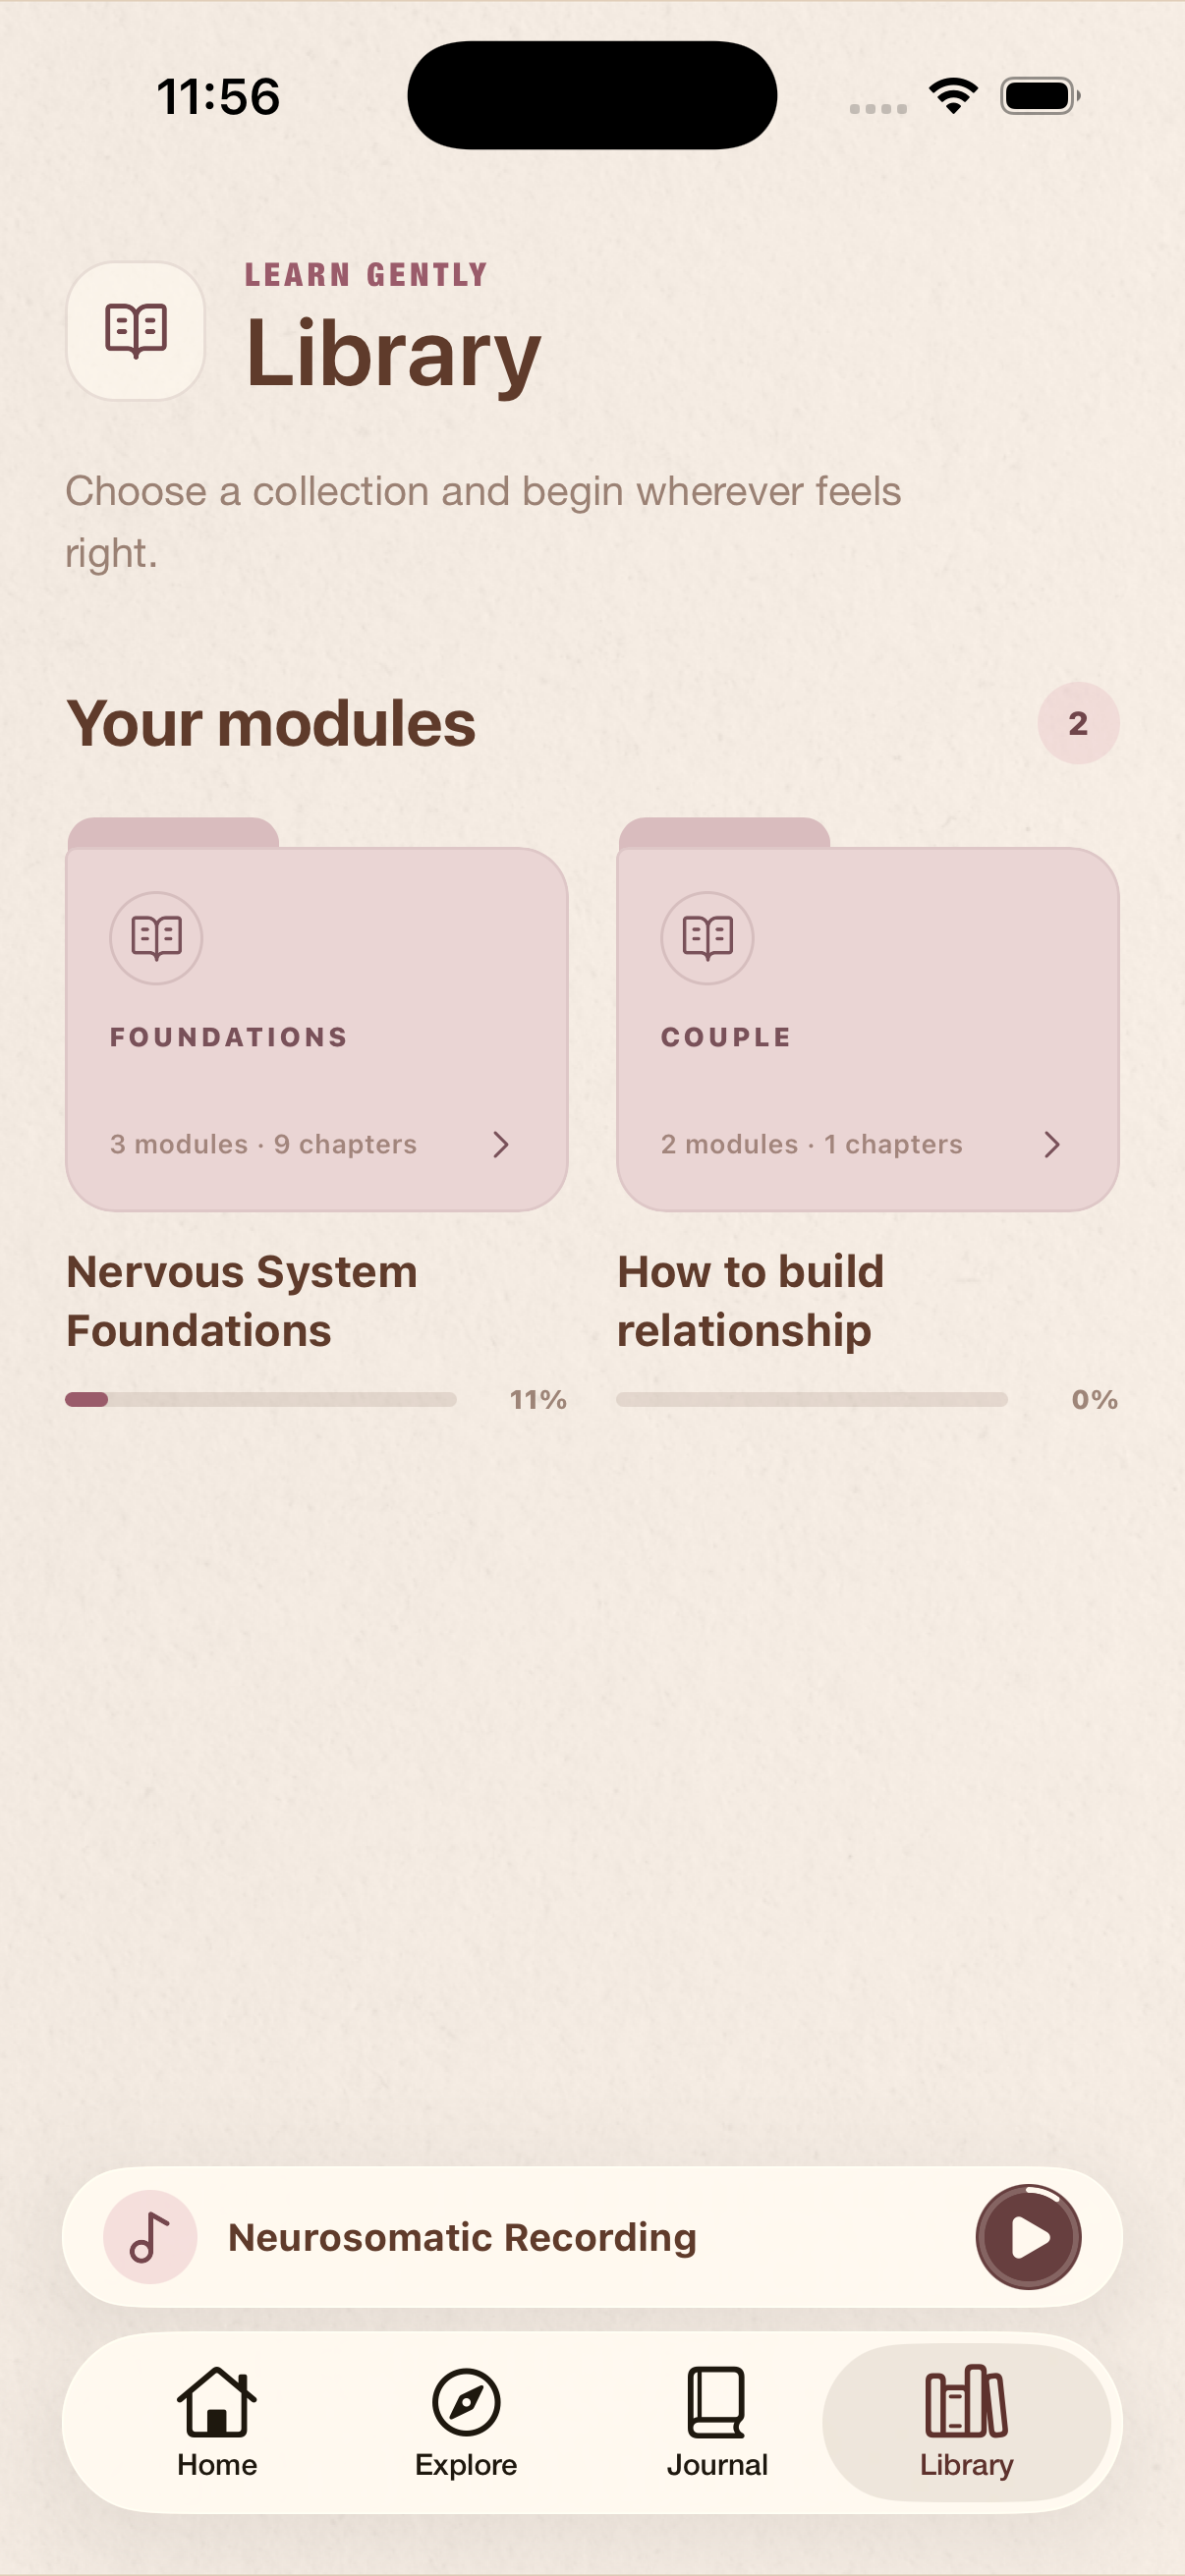
\includegraphics[width=\linewidth,height=0.62\textheight,keepaspectratio]{figures/library.png}
\caption[Library screen]{Existing iOS simulator Library screen, captured 3 October 2026. Course progress and the persistent compact audio player demonstrate implemented presentation features.}
\label{fig:library}
\end{figure}
\FloatBarrier

\subsection{Authentication and persistence}

The backend owns account identity and stores private records under that identity. Passwords are hashed, session storage uses native secure storage, and authenticated routes apply account-specific queries. Email verification, password recovery, password change, and account deletion have dedicated flows. Google identity-token verification is present in source, with native and backend configuration requirements. Apple identity handling remains for compatibility, while its sign-in controls were removed from the mobile authentication screens on 3 October 2026. Current provider implementation does not establish a completed production-signed login test.

PostgreSQL separates structured data from hosted media. Onboarding supplies a support goal, check-ins supply present context, and recommendation requests record returned items and associated context. Feedback and event records retain evidence for later adaptation. Persistence is especially important across app restarts, but it also introduces retention and deletion responsibilities. Account deletion can remove server-linked records and attempt local-key cleanup; it cannot erase a recovery key copied elsewhere or material retained outside the application's control.

\subsection{Five-stage hybrid recommendation engine}

The Node recommendation route loads onboarding, the latest check-in, eligible published exercise records, interaction aggregates, discomfort exclusions, and recent recommendation IDs. It rejects generation when required context is unavailable. User identifiers are transformed with an HMAC before being sent to the Python service. This reduces direct identifier exposure across that boundary, but the transformed identifier still links interactions within the service. Pseudonymisation is therefore not equivalent to anonymous data.

The Python engine loads its tokenizer and ONNX model, truncates input at the configured limit, pools token outputs when needed, and normalises embeddings. Scoring records component values and returns an explanatory reason. Collaborative activation requires at least two qualifying neighbours and at least two common interactions under current defaults. Without those conditions, the engine labels its strategy as content-based cold start. The saved benchmark exercises this cold-start pathway and cannot support conclusions about collaborative quality.

The application also has a local fallback recommendation algorithm for service failure. It shares comfort mapping with backend policy, but it is a different ranker from the Python benchmark. A successful empty response is preserved rather than refilled with unfiltered local suggestions. This distinction is important: degraded operation may justify alternate ranking, while an empty eligible set should continue to communicate that no suitable items were available under current constraints.

The interaction aggregation also deserves scrutiny. Current backend code combines explicit feedback and event values over a bounded recent period, groups them by user and exercise, and limits the returned interaction dataset. Averaging is simple to inspect, but may suppress disagreement between a completed activity and an uncomfortable experience. Sparse observations, repeated clicks, and differences in how users provide ratings can distort neighbour similarity. Future analysis should examine these behaviours before adjusting weights or increasing the influence of collaboration. A pseudonymous identifier helps separate the service from direct account identifiers, but does not remove the sensitivity of the behavioural record.

\subsubsection{Pipeline overview and service integration}
\label{sec:five-stages}

The project's recommendation workflow has five logical stages: (1) eligibility filtering, (2) suitability rules, (3) semantic matching, (4) collaborative signals, and (5) final ranking and explanation. These stages describe responsibilities rather than five independently deployed services. The Node API constructs the request and the Python service implements filtering and ranking. Within \texttt{recommend()}, vector encoding and neighbour estimation are calculated before the per-item score loop; the stage numbering below is an explanatory decomposition of that function, not a claim about its literal line-by-line execution order. Figure~\ref{fig:recommendation-five-stages} connects these responsibilities to the feedback loop.

\subsubsection{Stage 1: construct and filter the eligible candidate set}
\label{sec:stage-one}

The authenticated API loads the latest check-in, onboarding support goal, published recommendation-enabled exercises, behavioural aggregates, discomfort exclusions, and recent recommendation identifiers. A missing check-in produces an HTTP~409 response; an empty published catalogue produces HTTP~503. The API does not accept a client-supplied account identifier as authority for accessing private context. It converts identifiers to HMAC-SHA256 pseudonyms before the Python request. The current request explicitly contains \texttt{journal\_texts: []}; neither journal plaintext nor journal embeddings are uploaded for ranking.

The check-in supplies six dimensions: state, body, energy, stress, focus, and support. Optional comfort choices are mapped through a shared policy. Self-touch avoidance excludes the butterfly hug and self-containment hold; breath-hold avoidance excludes box breathing and candidates marked as requiring holds; head/eye scanning avoidance excludes orienting; inward body-scan avoidance excludes body scanning. These restrictions belong to the latest check-in. Separately, exercises previously reported as uncomfortable are excluded through account-specific feedback records.

Python's \texttt{eligible\_candidates()} deduplicates IDs, removes the explicit exclusion set, and applies \texttt{contraindication\_reasons()}. Signals are normalised before comparison with metadata. The existing high-activation policy removes breath-hold exercises when the reported state is anxious or overwhelmed, or stress is very stressed. These are implemented suitability policies, whose completeness depends on the declared inputs and content metadata. They are not an automated clinical assessment.

Let $E$ be the published candidate set, $X_u$ the explicit and discomfort-derived exclusions, and $Q(e,u)$ the implemented metadata/high-activation rejection predicate. The eligible set is
\begin{equation}
 E_u = \{e\in E: e\notin X_u \text{ and } \neg Q(e,u)\}.
 \label{eq:eligibility}
\end{equation}
Only $E_u$ proceeds to scoring and fresh-item selection. An exercise cannot regain eligibility through a high embedding score, a positive peer rating, or a need to fill four slots. If $E_u$ is empty, the engine returns an empty list with \texttt{no-candidates}. This is a valid policy outcome rather than an instruction to relax restrictions.

\subsubsection{Stage 2: calculate structured suitability rules}
\label{sec:stage-two}

\texttt{\_rule\_evaluation()} compares normalised check-in answers with an exercise's recommendation tags, support goals, and intended states. The field contributions are support~0.34, state~0.22, body~0.12, energy~0.10, stress~0.10, and focus~0.08. They sum to~0.96; they are not a probability distribution. Additional adjustments consider activation level and physical intensity. For example, a down-regulating exercise receives~0.12 for a calm-down support match and~0.10 for an anxious/overwhelmed state. Up-regulating activities receive~0.14 for an energy support match. High-intensity activity is penalised by~0.38 for tired/drained energy; moderate intensity is penalised by~0.10 in that condition. The resulting rule score is clipped to $[0,1]$.

Writing $m_j(e,u)$ for a metadata match in field $j$, $w_j$ for its contribution, and $\Delta(e,u)$ for the implemented adjustments gives
\begin{equation}
 R(e,u)=\operatorname{clip}_{[0,1]}\!\left(\sum_j w_jm_j(e,u)+\Delta(e,u)\right).
 \label{eq:rule-score}
\end{equation}
Hard eligibility and soft ranking adjustments have distinct purposes. A metadata contraindication causes removal in Stage~1; a moderate-intensity penalty can instead reorder otherwise eligible items. The returned matched fields also support explanation text. These transparent heuristics are defensible as inspectable implementation choices, but the present benchmark does not independently validate every weight or suitability interpretation.

\subsubsection{Stage 3: compare meaning using MiniLM embeddings}
\label{sec:stage-three}

The engine constructs three kinds of document: the current check-in context, the goal/history context, and one description per eligible exercise. Exercise descriptions concatenate title, category, description, recommendation tags, support goals, intended states, activation level, and intensity. The current context uses labelled check-in answers. Although the Python schema retains a history-document function for older evaluation fixtures, the current application supplies no journals; the live history component uses the onboarding goal when present.

The pretrained \texttt{all-MiniLM-L6-v2} tokenizer truncates inputs at 256 tokens. ONNX Runtime executes the model on the CPU. When inference returns token-level vectors, attention-mask-weighted mean pooling excludes padding; sentence-level outputs are used directly. Embeddings are converted to NumPy arrays, checked for expected shape, and normalised. Current-context similarity $C$ and goal/history similarity $H$ use the clipped cosine comparison
\begin{equation}
 C(e,u)=\operatorname{clip}_{[0,1]}\!\left(\frac{\mathbf v_e\cdot\mathbf v_c}{\|\mathbf v_e\|\,\|\mathbf v_c\|}\right),\qquad
 H(e,u)=\operatorname{clip}_{[0,1]}\!\left(\frac{\mathbf v_e\cdot\mathbf v_h}{\|\mathbf v_e\|\,\|\mathbf v_h\|}\right).
 \label{eq:semantic-score}
\end{equation}
If the goal/history document is empty, the code still encodes that document; it does not explicitly disable the five-percent history term. This is a concrete implementation limitation worth considering in a future ablation. The model is pretrained rather than trained or fine-tuned on the project's users. It measures descriptive similarity and does not generate therapeutic advice.

If model loading or inference fails, production Python can use deterministic, 384-dimensional hashed token counts. SHA256 assigns tokens to dimensions, after which vectors are normalised. This lexical fallback is labelled in the model backend and logs the error class without user text. Strict ONNX evaluation disables fallback, so a failed model cannot silently produce a benchmark described as semantic inference. The separate mobile fallback is another algorithm and should not inherit the measured accuracy of the Python ranker.

\subsubsection{Stage 4: add collaborative evidence only when sufficient history exists}
\label{sec:stage-four}

The API maps exercise events to bounded preference values: opened~0.15, started~0.35, completed~0.80, saved~0.70, repeated~1.00, and abandoned~$-0.40$. Explicit feedback takes precedence within its own record: uncomfortable maps to~$-1.00$; worse to~$-0.75$; better to~$1.00$; otherwise helpfulness $h\in\{0,1,2,3\}$ maps to $h/1.5-1$. The backend averages combined feedback/event observations per user and exercise over 180 days, clips to $[-1,1]$, and retrieves at most 10,000 aggregate rows. The feedback and event records can therefore counterbalance one another. An uncomfortable exercise nevertheless remains an explicit exclusion for that account, regardless of its averaged value.

User--user cosine similarity is calculated only over jointly interacted exercise IDs. A qualifying neighbour must have at least two common items and positive cosine similarity. At least two qualifying neighbours activate collaboration under the defaults. For an eligible exercise, the component is
\begin{equation}
 B(e,u)=\frac{1}{2}\left(1+\frac{\sum_{v\in N_u(e)}\operatorname{sim}(u,v)r_{v,e}}{\sum_{v\in N_u(e)}\operatorname{sim}(u,v)}\right),
 \label{eq:collaborative-score}
\end{equation}
where $N_u(e)$ contains qualifying neighbours with an observation for $e$. A missing collaborative estimate defaults to~0.5 when collaboration is active. Without enough neighbours, the collaborative contribution is disabled and the returned strategy is \texttt{content-based-cold-start}. This allows a new user to receive suggestions from current context and content metadata.

Feedback changes future inputs; it does not retrain MiniLM after every event. Moreover, a completion event can reflect persistence rather than helpfulness, and two positive-similarity neighbours provide limited evidence. The current saved benchmark has no interaction histories and therefore tests the cold-start path, not the accuracy or fairness of collaborative recommendations.

\subsubsection{Stage 5: blend, rotate, diversify, explain, and persist}
\label{sec:stage-five}

The base blend switches according to collaborative availability:
\begin{align}
 S_{\mathrm{cold}}(e,u)&=0.72R+0.23C+0.05H,\label{eq:cold-start}\\
 S_{\mathrm{warm}}(e,u)&=0.65R+0.20C+0.05H+0.10B.\label{eq:warm-start}
\end{align}
Figure~\ref{fig:recommendation-weights} shows both modes. An earlier diagram's single 65/25/10 split combines current and goal/history similarity and describes only the collaboration-active blend. It does not represent cold-start weights. The revised account separates both semantic terms and both modes.

\begin{figure}[htbp]
\centering
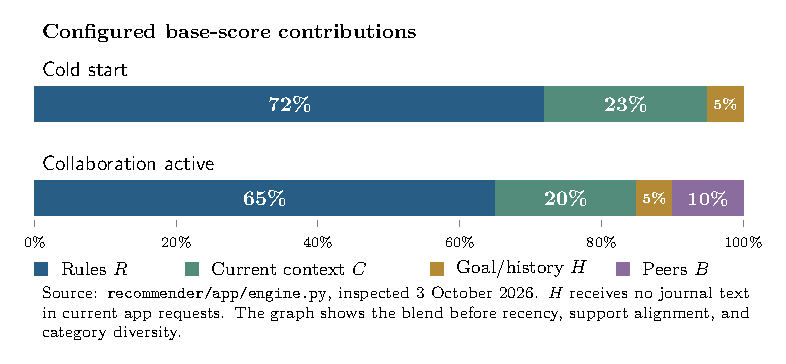
\includegraphics[width=\linewidth,height=0.62\textheight,keepaspectratio]{figures/recommendation-weights.pdf}
\caption[Cold-start and collaboration-active score weights]{Implemented score-component weights in cold start and collaboration-active mode. These are configured ranking contributions, not measured causal importance or success probabilities.}
\label{fig:recommendation-weights}
\end{figure}
\FloatBarrier

The API supplies up to 24 recent item impressions from a 14-day window, excluding requests tied to the same latest check-in. Python approximates request age by each item's index divided by the requested list size. Each impression contributes $0.18\times0.72^a$, with accumulated penalty capped at~0.42. The preselection score is $\max(0,S-P_{\mathrm{recency}})$. This provides gentle rotation, although reconstructing age from item order is approximate when historical lists are shorter than four.

Candidate ordering begins with descending score and exercise-ID tie breaking. If at least four eligible items align with the primary support goal, selection restricts to that pool; otherwise the full eligible set remains available. If enough candidates have recency penalties below $0.9\times0.42$, that less-exposed pool is preferred. Greedy selection then maximises the stored score minus~0.08 for each already selected item in the same category. Category diversity therefore affects positions, but the stored score does not include this per-selection diversity subtraction.

If a complete selected set would repeat the most recent set, only the final slot may be replaced with an unseen, eligible, support-aligned item. That item is marked as exploration. No separate minimum semantic-similarity threshold is enforced in this substitution, so its appropriateness still needs longitudinal evaluation. Normal results contain up to four exercises, score components, reasons, and the exploration flag. Reasons follow deterministic matched-field templates; they explain a declared match and do not provide a complete attribution of every score contribution.

The Node API saves the request, context flags, ordered items, and impression events within a database transaction. Ownership checks govern subsequent feedback. The Home screen maps returned IDs to mobile-renderable exercises and ignores unmapped IDs, another reason fewer than four cards can appear. A successful empty response is preserved. A request failure activates the local TypeScript ranker, which shares comfort filtering but does not receive the server's full persistent discomfort, collaborative, or recency history.

\subsubsection{Worked scoring example and algorithm summary}
\label{sec:worked-recommendation}

Consider an illustrative eligible grounding exercise with $R=0.80$, $C=0.60$, and $H=0.40$. Its cold-start base score is $0.72(0.80)+0.23(0.60)+0.05(0.40)=0.734$. One newest-request impression subtracts~0.18, producing~0.554. If a category peer has already been selected, its selection utility becomes~0.474 after the diversity deduction, while the recorded score remains~0.554. These inputs are deliberately illustrative and are not a measured user case. If the same exercise were explicitly excluded in Stage~1, none of these calculations could return it.

\begin{lstlisting}[caption={Five-stage algorithm summary. Operational logging and ownership checks occur in the API around this ranker.},label={lst:five-stage-algorithm}]
1  context <- authenticated check-in, goal, catalogue, activity
2  eligible <- deduplicate and apply all known exclusions
3  if eligible is empty: return an empty result
4  R <- structured suitability for each eligible exercise
5  C, H <- semantic similarities; journals remain absent
6  B, active <- positive neighbours with sufficient overlap
7  S <- cold blend, or warm blend when active
8  subtract recency; prefer support-aligned eligible options
9  greedily diversify; conditionally replace only final slot
10 return up to four items with reasons and components
11 persist request/items/impressions; accept owned feedback
\end{lstlisting}

The explanation is grounded in \path{backend/src/routes/recommendations.ts}, \path{backend/src/data/comfortPreferences.ts}, \path{recommender/app/engine.py}, \path{src/services/recommendations/recommendationEngine.ts}, and \path{src/screens/home/HomeScreen.tsx}, inspected on 3 October 2026. Equations~\ref{eq:eligibility}--\ref{eq:warm-start} express implemented operations; future weight tuning, independent content review, and collaborative evaluation remain research tasks.


\subsection{Encrypted journaling}

Journal creation begins with vault setup and recovery-backup confirmation. Entry titles, prompts, packs, and text are serialised and encrypted locally. The backend accepts versioned ciphertext envelopes and rejects new plaintext writes. On retrieval, the device decrypts content only after unlocking. Wrong-account, wrong-key, altered-ciphertext, and identifier mismatches should fail authentication rather than display plausible corrupted text. Current source also defines authenticated encryption for journal media, with its own associated identifiers and media purpose.

\begin{figure}[htbp]
\centering
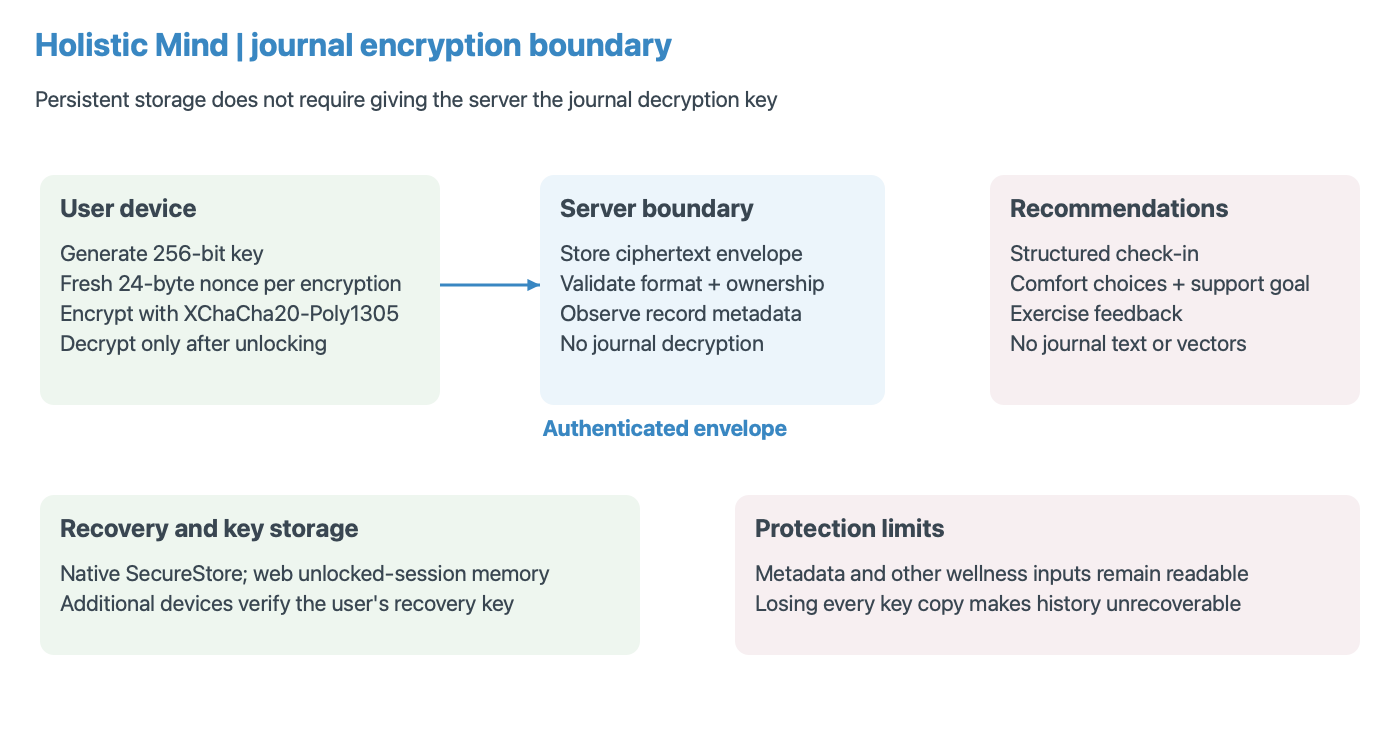
\includegraphics[width=\linewidth,height=0.62\textheight,keepaspectratio]{figures/privacy.png}
\caption[Journal encryption and recovery boundary]{Journal encryption and recovery boundary. The server stores envelopes and metadata; journal text and decryption keys are excluded from recommendation requests.}
\label{fig:privacy}
\end{figure}
\FloatBarrier

Legacy migration is explicit rather than a silent server-side conversion. An unlocked client retrieves older entries, encrypts and verifies them, and submits conditional replacements. The previous plaintext fields become null while the original record identity and timestamp remain. Retrying a migration should return the already encrypted result without overwriting it. The documented tests used synthetic entries and did not migrate real journals. A production transition must also address retained backups and compatibility with older clients.

\subsection{Content administration and deployment}

The administration application manages exercises, audio records, curriculum structure, and related media through protected backend operations. Published status controls ordinary content availability, while recommendation metadata adds intended states, support goals, activation levels, and restrictions. This allows presentation content and ranking semantics to evolve together. However, inaccurate metadata can undermine eligibility even when upload, authentication, and publication mechanisms operate correctly. Content review is consequently part of maintaining recommendation quality.

Local development uses containerised PostgreSQL, object storage, and the recommendation service alongside the API and mobile tooling. Deployment documentation describes managed database, private service networking, S3-compatible hosting, and configured email delivery. These are reproducible operational arrangements, not evidence of full production acceptance. Export/\allowbreak{}import scripts support moving managed content between environments. Private wellness records should not be treated as content-promotion data, and no live deployment change was performed for this report.

\begin{figure}[htbp]
\centering
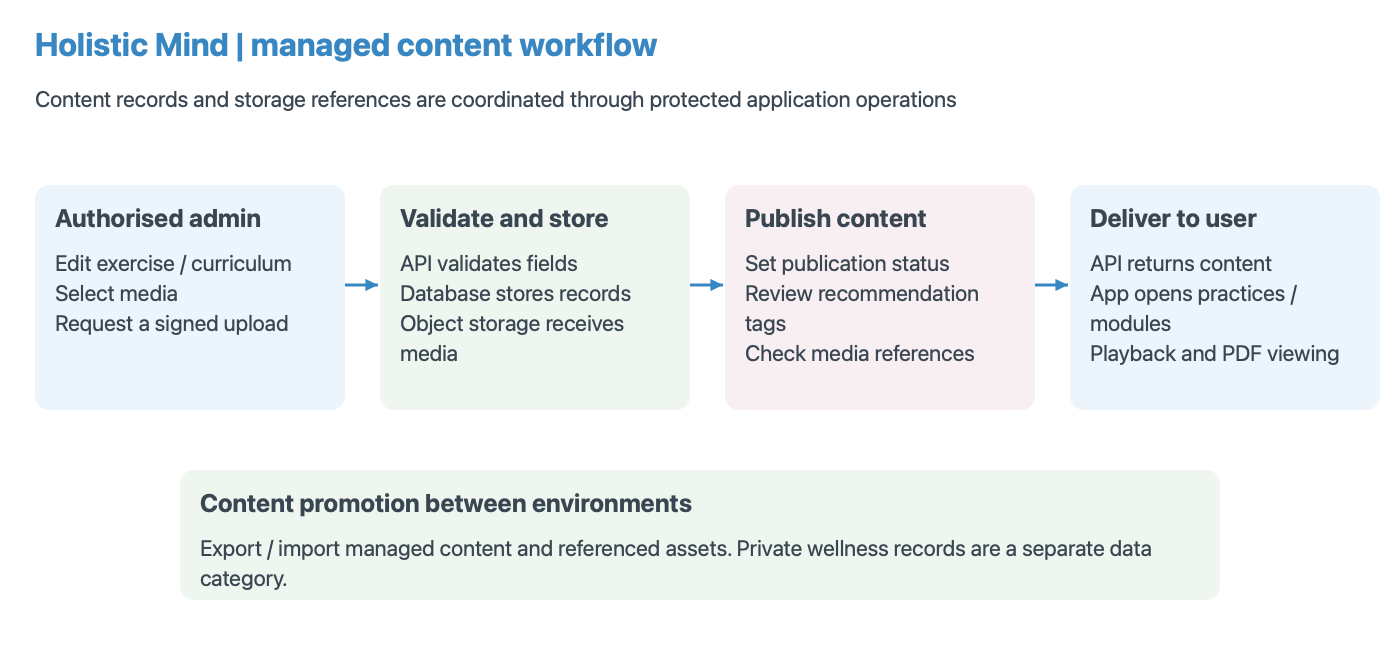
\includegraphics[width=\linewidth,height=0.62\textheight,keepaspectratio]{figures/content.png}
\caption[Content publication workflow]{Content publication workflow reconstructed from the implemented admin, API, and storage modules. A published record and usable media reference are distinct prerequisites for delivery.}
\label{fig:content}
\end{figure}
\FloatBarrier

\subsection{Screen-by-screen implementation}

The Home screen presents the daily check-in as the main action and follows it with suggested tools and progress information. The check-in stores six values: state, body, energy, stress, focus, and support. Comfort preferences are additional optional choices rather than a seventh inferred mental-health measurement. The final step can exclude self-touch, breath holds, head or eye scanning, and inward body scans. These choices apply to the stored check-in, so the user should not assume that they are permanent account-wide settings.

Explore provides independent access to exercise categories and available audio. A person can use it when no recommendation has been generated or when they prefer another activity. Exercise detail screens support the relevant guidance format, including timed breathing, guided material, and media playback. Recommendation feedback is associated with the returned practice context when available. Opening, starting, and completing are distinct events; none is treated as direct proof of benefit. Figure~\ref{fig:home_explore} shows earlier Home and Explore interfaces from the September progress review.

\begin{figure}[htbp]
\centering
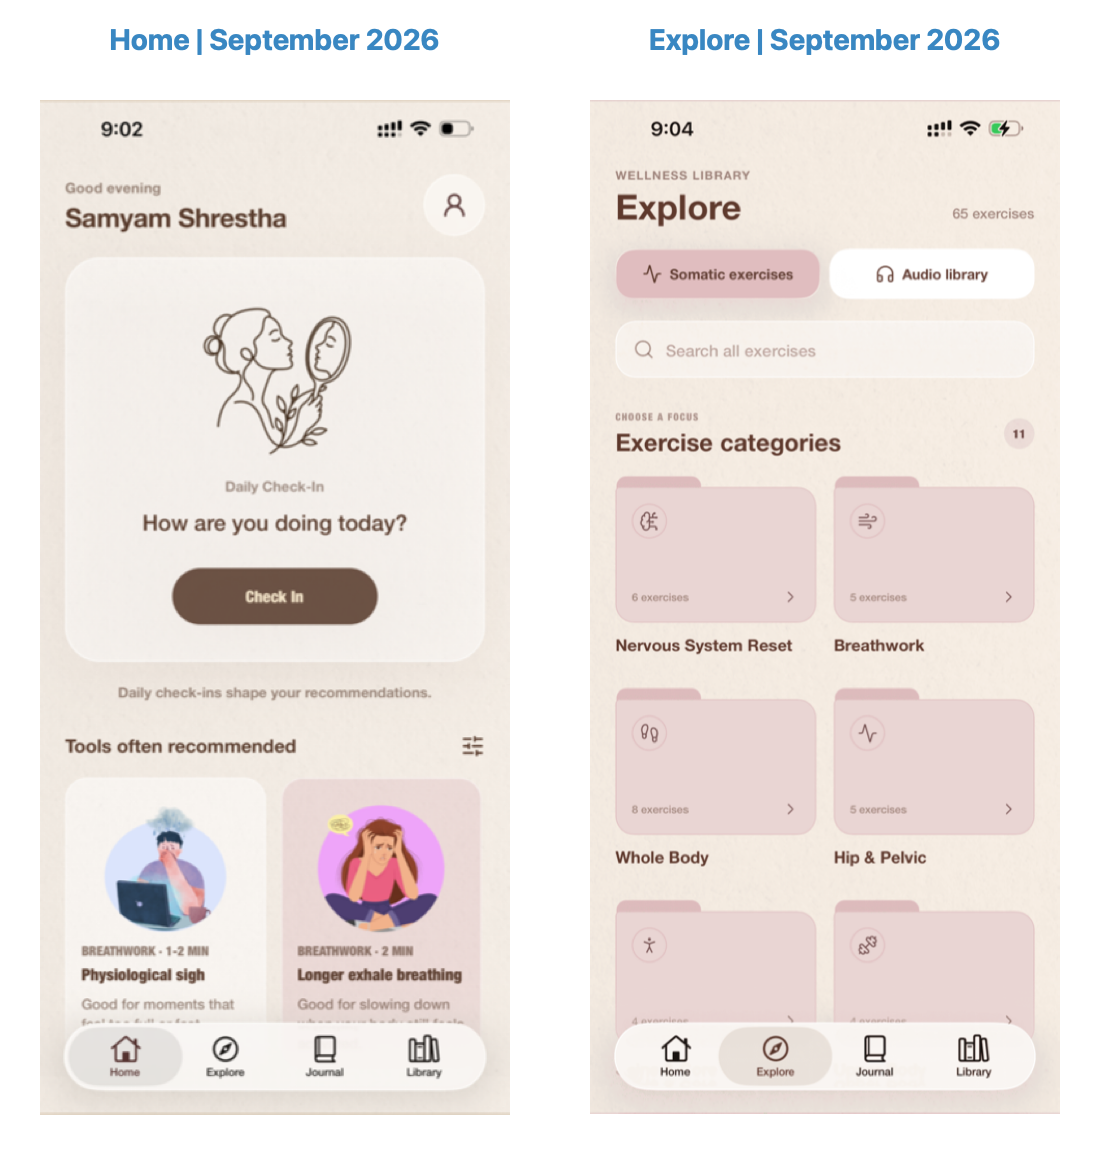
\includegraphics[width=\linewidth,height=0.62\textheight,keepaspectratio]{figures/home_explore.png}
\caption[Historical Home and Explore interfaces]{Historical Home and Explore interfaces reproduced from Shrestha's final progress review dated 2 September 2026. Catalogue counts and interface details describe that captured version.}
\label{fig:home_explore}
\end{figure}
\FloatBarrier

Journal supports prompted packs and free writing behind an unlock/\allowbreak{}setup gate. The free-writing editor manages title, text, attachments, save state, and unsaved changes. Navigation away from a draft asks whether it should be discarded. The current Journal security page centralises recovery and locking controls rather than placing a large control panel beneath every journal or history view. This refinement reduces visual clutter while keeping sensitive operations accessible through Profile.

Profile groups account details, password/\allowbreak{}security actions, preferences, reminders, and history. History brings together recorded check-ins, practice information, and reflections that can be decrypted while the vault is unlocked. The September screenshots show an earlier form of those screens (Figure~\ref{fig:history_profile}). The report uses them as development evidence, not as proof that every current control has been exercised on a physical device. The captions preserve that date so interface history does not become an implicit release certification.

\begin{figure}[htbp]
\centering
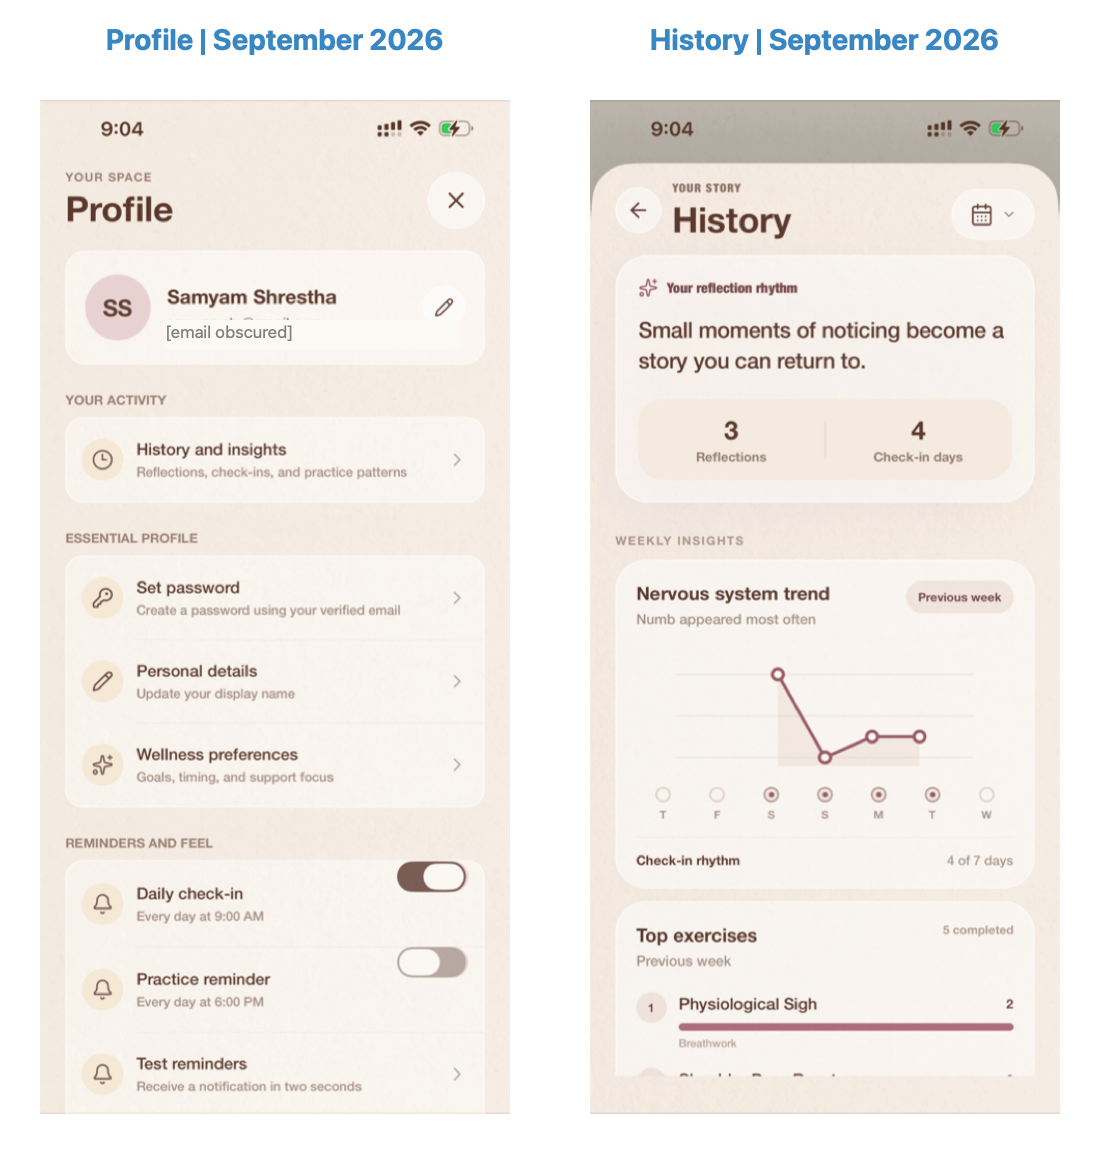
\includegraphics[width=\linewidth,height=0.62\textheight,keepaspectratio]{figures/history_profile.png}
\caption[Historical Profile and History interfaces]{Historical Profile and History screens from the 2 September 2026 progress review. The account email is obscured for presentation; journal security controls have since been reorganised.}
\label{fig:history_profile}
\end{figure}
\FloatBarrier

\subsection{Curriculum and audio implementation}

The learning Library is distinct from the short-practice catalogue. It uses courses, modules, and chapter records to organise longer material, with media and interactive chapter types defined in the backend. Section progress supports returning to a learning sequence. AudioPlayerContext provides a shared player state, and a compact player remains available across appropriate screens. This design avoids requiring the user to reopen the originating screen simply to pause a recording.

PDF viewing is handled separately from video and audio playback, with native and web implementations. The current code also includes interactive questions and multiple-choice content structures. Their availability allows the administrator to mix explanatory text, media, and participation within a course. It does not prove that the educational sequence has been assessed for learning effectiveness. A course can be technically navigable while still needing editorial review of its pacing, wording, and intended audience.

For usability, playback should remain predictable when navigating, receiving an interruption, or reopening the app. Those scenarios deserve native release testing because a web export cannot fully exercise platform audio behaviour. Likewise, successful PDF retrieval should be tested with large files, unsupported formats, and network errors. These priorities extend the final progress review's useful observation that apparently small interface defects can affect the overall experience.

\subsection{Authentication, provider configuration, and reminders}

Password hashing uses Argon2id in the current backend. Session handling, verification codes, and recovery actions are separate from journal recovery. Google sign-in requires matching native and backend client configuration as well as a reachable application API. The 3 October change record describes a simulator network failure caused by a stopped API and a new readiness check that presents a more specific failure message. It also states that a complete Google login still needs user retry. A configured provider should therefore not be described as end-to-end verified merely from source inspection.

Apple sign-in controls were removed from current login and signup screens on 3 October. Backend identity handling remains for existing Apple-linked accounts and account deletion. This corrects the earlier report's broader account-feature description. The final artefact should be documented at its current visible capability, with retained backend compatibility explained separately. It would be misleading to list Apple sign-in as a present mobile action simply because provider verification code remains in the repository.

Reminder scheduling uses Expo Notifications and local daily triggers when permission is granted. Current code schedules the daily check-in at 09:00 and practice at 18:00, with Android channel handling and a test reminder. The onboarding's preferred time is a separate stored value; its presence does not establish fully custom reminder scheduling. Web does not use these native local notifications. A release test should verify permission refusal, setting changes, cancellation on logout, and behaviour across device time changes.

\subsection{Journal media and atomicity}

Current source extends reflection beyond text through encrypted image and audio attachments. Media encryption binds the account, media identifier, key identifier, kind, content type, and entry association into authenticated data. This protects against substituting encrypted bytes into a different purpose or record. The journal context and attachment composer coordinate the draft, while the backend validates encrypted media and supports a combined entry-and-media operation. Encrypted user media is distinct from ordinary published exercise media.

The with-media endpoint uses a database transaction for the entry and related attachment records, allowing the server-side write to succeed or roll back as a unit. Client state still matters: recording, selecting an image, encryption, network transfer, and retry can fail before that transaction begins. The server's atomicity does not protect an unsaved local draft from being deliberately discarded. Tests should distinguish these stages rather than interpreting one transaction check as a complete attachment-workflow validation.

\subsection{Deployment evolution and release status}

The September final progress review reports a beta deployment using Railway, Vercel, and Cloudflare R2 alongside local Docker services. It also reports managed-content export/\allowbreak{}import without private user data. This is valuable historical evidence and should be retained. The report preparation did not independently query those deployments, inspect release logs, or exercise their live account operations. Later local encryption and security refinements therefore have their own validation and rollout boundaries.

A release of the present source requires coordinated backend schema, journal API, and native application versions. The latest encrypted clients expect envelope-based writes, while older plaintext clients are incompatible with that contract. Media configuration, API readiness, private recommender networking, email delivery, and native provider settings also require environment-specific checks. These are operational dependencies of the implemented system, not new features promised by this dissertation.

Figure~\ref{fig:evolution} summarises the main changes across the supplied reports and repository records. It shows the shift from a proposed Firebase-backed app to a relational multi-service platform, followed by stronger comfort and journal boundaries. The graphic is evidence of documented design evolution. It is not an independent verification of every historical deployment claim or an assertion that the proposed participant study has been completed.

\begin{figure}[htbp]
\centering
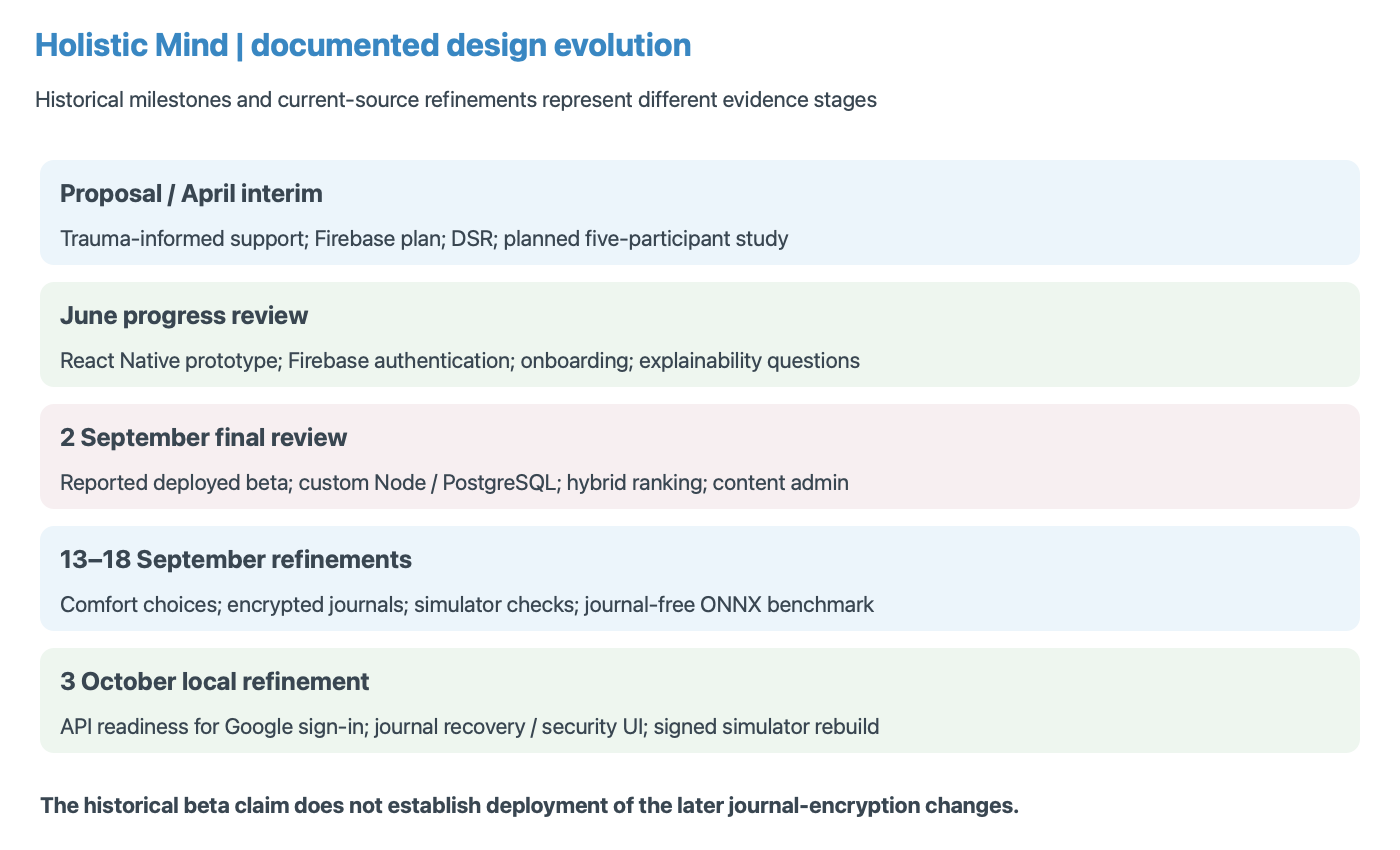
\includegraphics[width=\linewidth,height=0.62\textheight,keepaspectratio]{figures/evolution.png}
\caption[Evolution of the implemented design]{Project evolution across the April and June submissions, September final review, and later local refinements. Reported beta deployment and current encryption rollout are shown as distinct stages.}
\label{fig:evolution}
\end{figure}
\FloatBarrier

\clearpage\section{Validation and Testing}\label{sec:chapter-7}

\subsection{Test strategy and evidence boundaries}

Validation combines saved evaluation outputs, regression-test source, and an existing device-and-backend test record. The report does not claim that these suites were newly rerun during preparation. The functional record is dated 15 September 2026 and describes an iPhone simulator with local Node, PostgreSQL, and Docker recommendation services. That provides useful integration evidence, while leaving physical-device behaviour, production configuration, and full automated native screen coverage unresolved.

Different checks address different failure classes. Ranking metrics quantify agreement with authored relevance labels. Explicit-exclusion tests check whether declared policy is preserved. Cryptographic tests examine round trips and tampering failures. API checks examine ownership and accepted formats. Native checks address module availability, secure key storage, restart persistence, and connectivity. A good score in one layer cannot substitute for a missing check in another, so the conclusions preserve these evidence boundaries.

\subsection{Journal-free ranking benchmark}

The journal-free ONNX run was generated on 18 September 2026 using hybrid-v4, the MiniLM ONNX backend, 30 scenarios, ten repeats per approach, and seed 42. Four approaches were compared: random ranking, semantic text similarity, rules with eligibility, and the hybrid. All deduplicate and honour explicit exercise exclusions, but random and text-only do not apply the same suitability rules as rules and hybrid. This is a comparison of complete approaches, not a controlled ablation isolating one component.

Relevance is defined as an authored label of at least two. Precision@4 divides relevant returned items by four, penalising unfilled slots. NDCG@4 uses graded gains and rank discounts to compare the returned ordering with an ideal ordering. Negative labels contribute zero gain but are also reported through a separate violation measure. Fill rate helps reveal systems that avoid violations simply by returning nothing. Bootstrap intervals resample the 30 scenario means; they estimate variation within this dataset rather than clinical or population uncertainty.

\begingroup
\small\setstretch{1.08}
\setlength{\tabcolsep}{4pt}
\setlength{\TableInnerWidth}{\dimexpr\linewidth-24pt\relax}
\begin{longtable}{@{}>{\raggedright\arraybackslash}p{0.340\TableInnerWidth} >{\raggedright\arraybackslash}p{0.200\TableInnerWidth} >{\raggedright\arraybackslash}p{0.200\TableInnerWidth} >{\raggedright\arraybackslash}p{0.260\TableInnerWidth}@{}}
\caption{Saved journal-free ONNX benchmark, 30 authored scenarios. Violation percentages represent negative benchmark labels, not measured adverse outcomes.}\label{tab:table-3}\\
\toprule
\textbf{Approach} & \textbf{Precision@4} & \textbf{NDCG@4} & \textbf{Negative-label items} \\
\midrule\endfirsthead
\multicolumn{4}{l}{\textit{Table \thetable\ continued}}\\
\toprule
\textbf{Approach} & \textbf{Precision@4} & \textbf{NDCG@4} & \textbf{Negative-label items} \\
\midrule\endhead
\midrule\multicolumn{4}{r}{\textit{Continued on next page}}\\\endfoot
\bottomrule\endlastfoot
Random & 48.50\% & 0.4315 & 5.17\% \\ \addlinespace[4pt]
MiniLM text similarity & 71.67\% & 0.6602 & 1.67\% \\ \addlinespace[4pt]
Rules + eligibility & 73.33\% & 0.7244 & 2.50\% \\ \addlinespace[4pt]
Hybrid & 77.50\% & 0.7387 & 3.33\% \\ \addlinespace[4pt]
\end{longtable}
\endgroup

The hybrid returned an average of 3.1 relevant items per four. Its precision exceeded rules by 4.17 percentage points and NDCG by 0.0143. Those improvements are modest and should be read alongside the higher negative-label rate. Text-only recorded fewer negative-labelled selections in this suite. Figure~\ref{fig:productionchart} includes quality and warm timing, making the trade-offs visible rather than selecting only the strongest hybrid metric. No statistical significance or clinical superiority is inferred from the point estimates.

\begin{figure}[htbp]
\centering
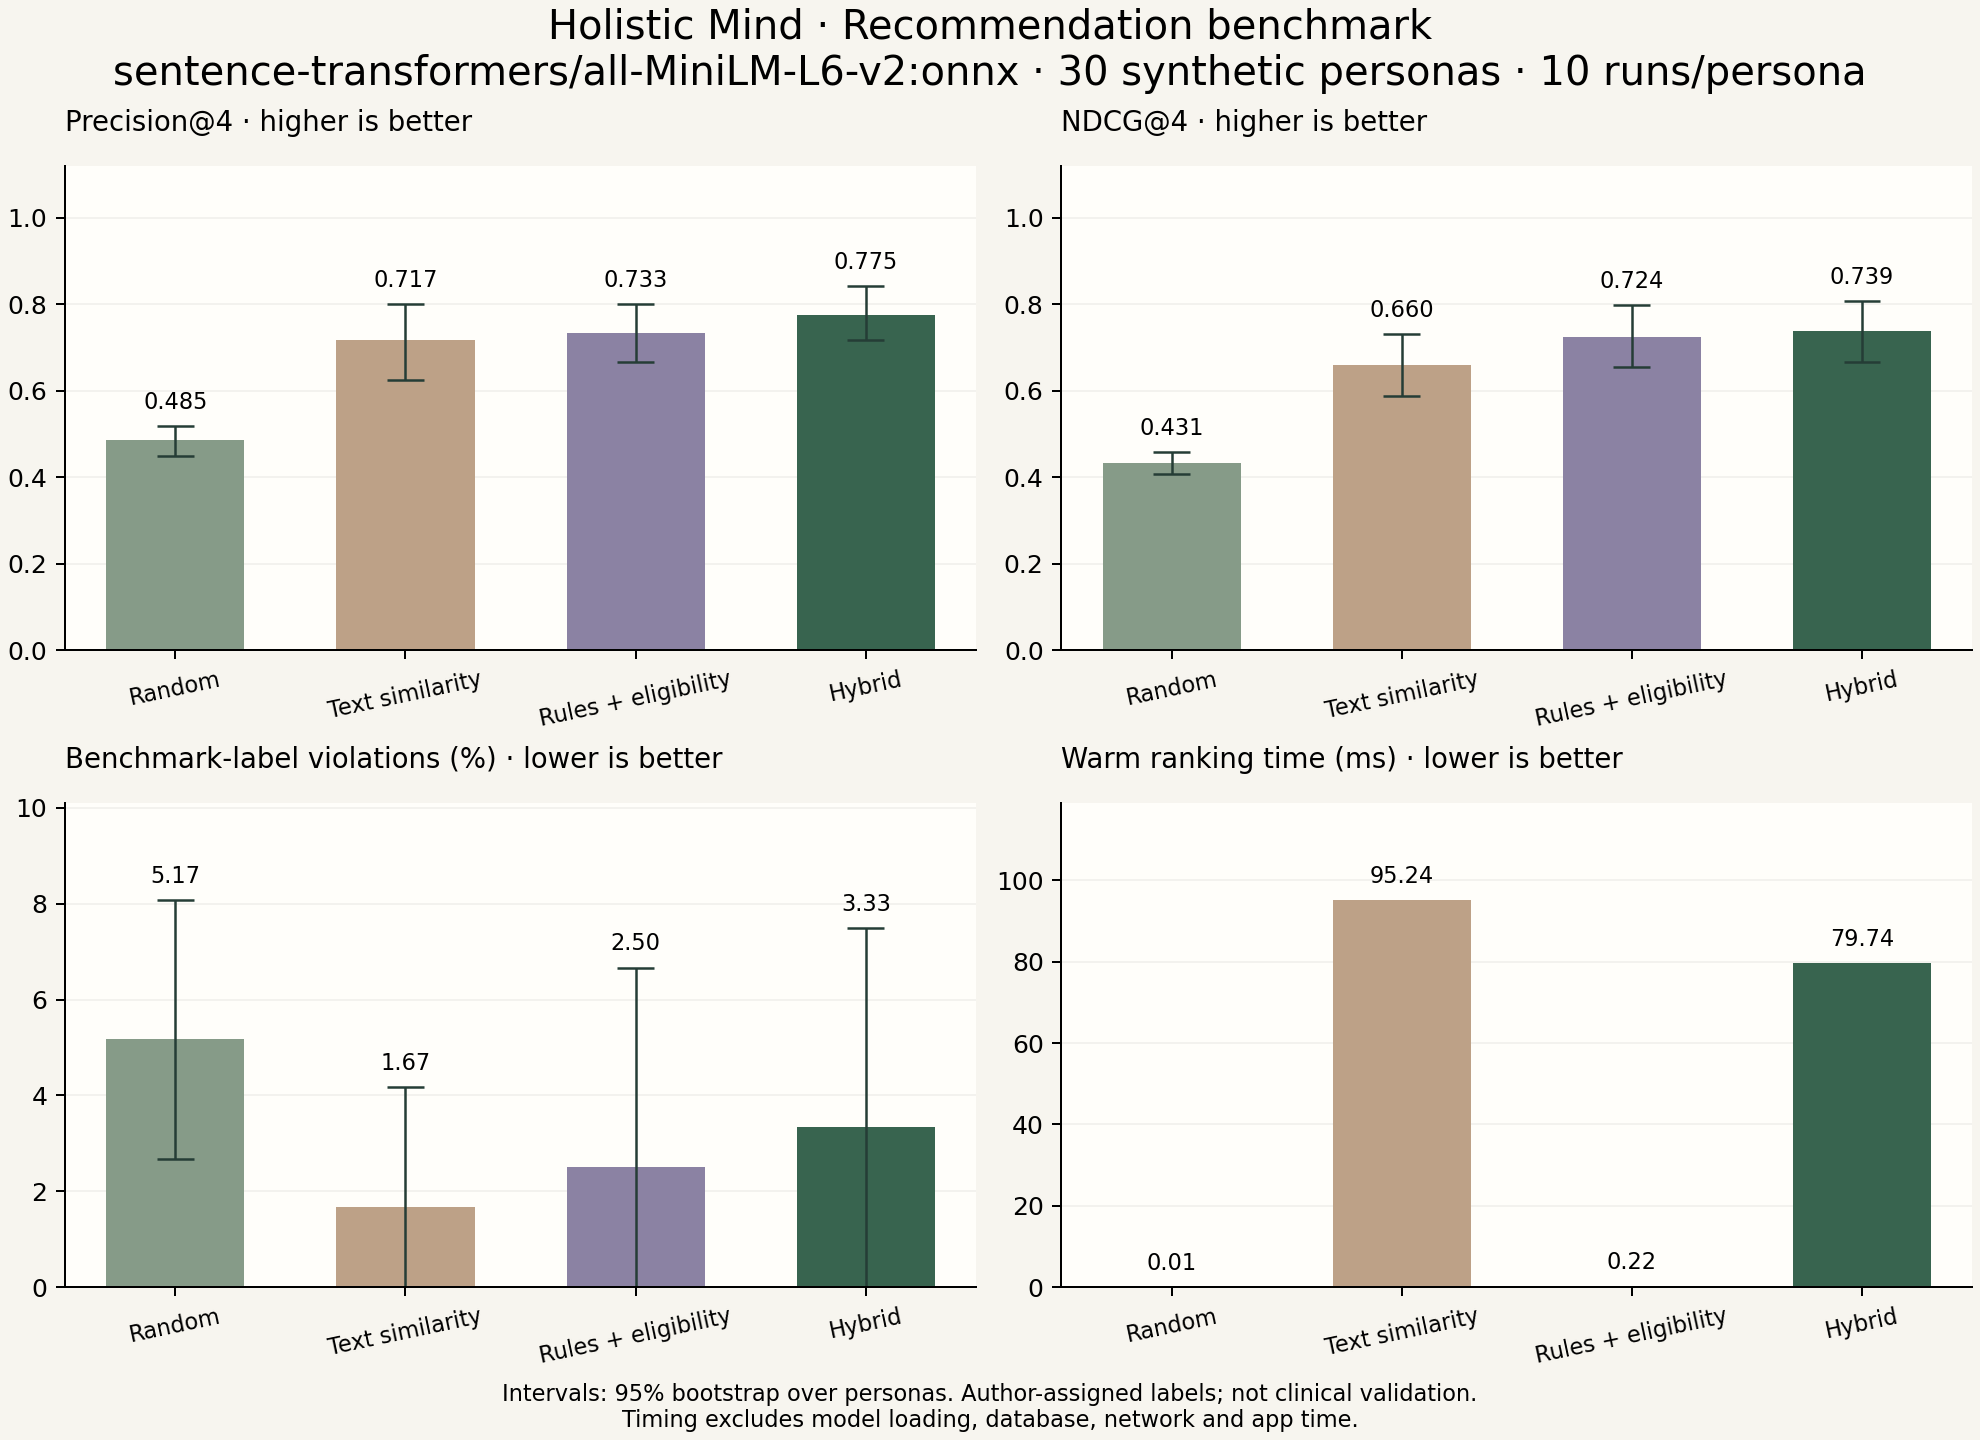
\includegraphics[width=\linewidth,height=0.62\textheight,keepaspectratio]{figures/productionchart.png}
\caption[Journal-free ONNX benchmark results]{Existing project benchmark chart for journal-free ONNX evaluation. Error bars are bootstrap intervals over authored scenarios; timing excludes startup, database, HTTP, and mobile rendering.}
\label{fig:productionchart}
\end{figure}
\FloatBarrier

\subsection{Comfort restrictions and unresolved cases}

The separate comfort suite contains eight selected variants with declared choices, including individual restrictions and combinations. All approaches recorded zero explicit exclusion violations with full top-four fill in these selected cases. Hybrid precision was 90.62\% and NDCG was 0.7441, while text-only NDCG was higher at 0.7885. These figures should not be compared directly with the 30-scenario benchmark because the comfort cases are a selected stress suite, sometimes derived from the same source persona.

\begin{figure}[htbp]
\centering
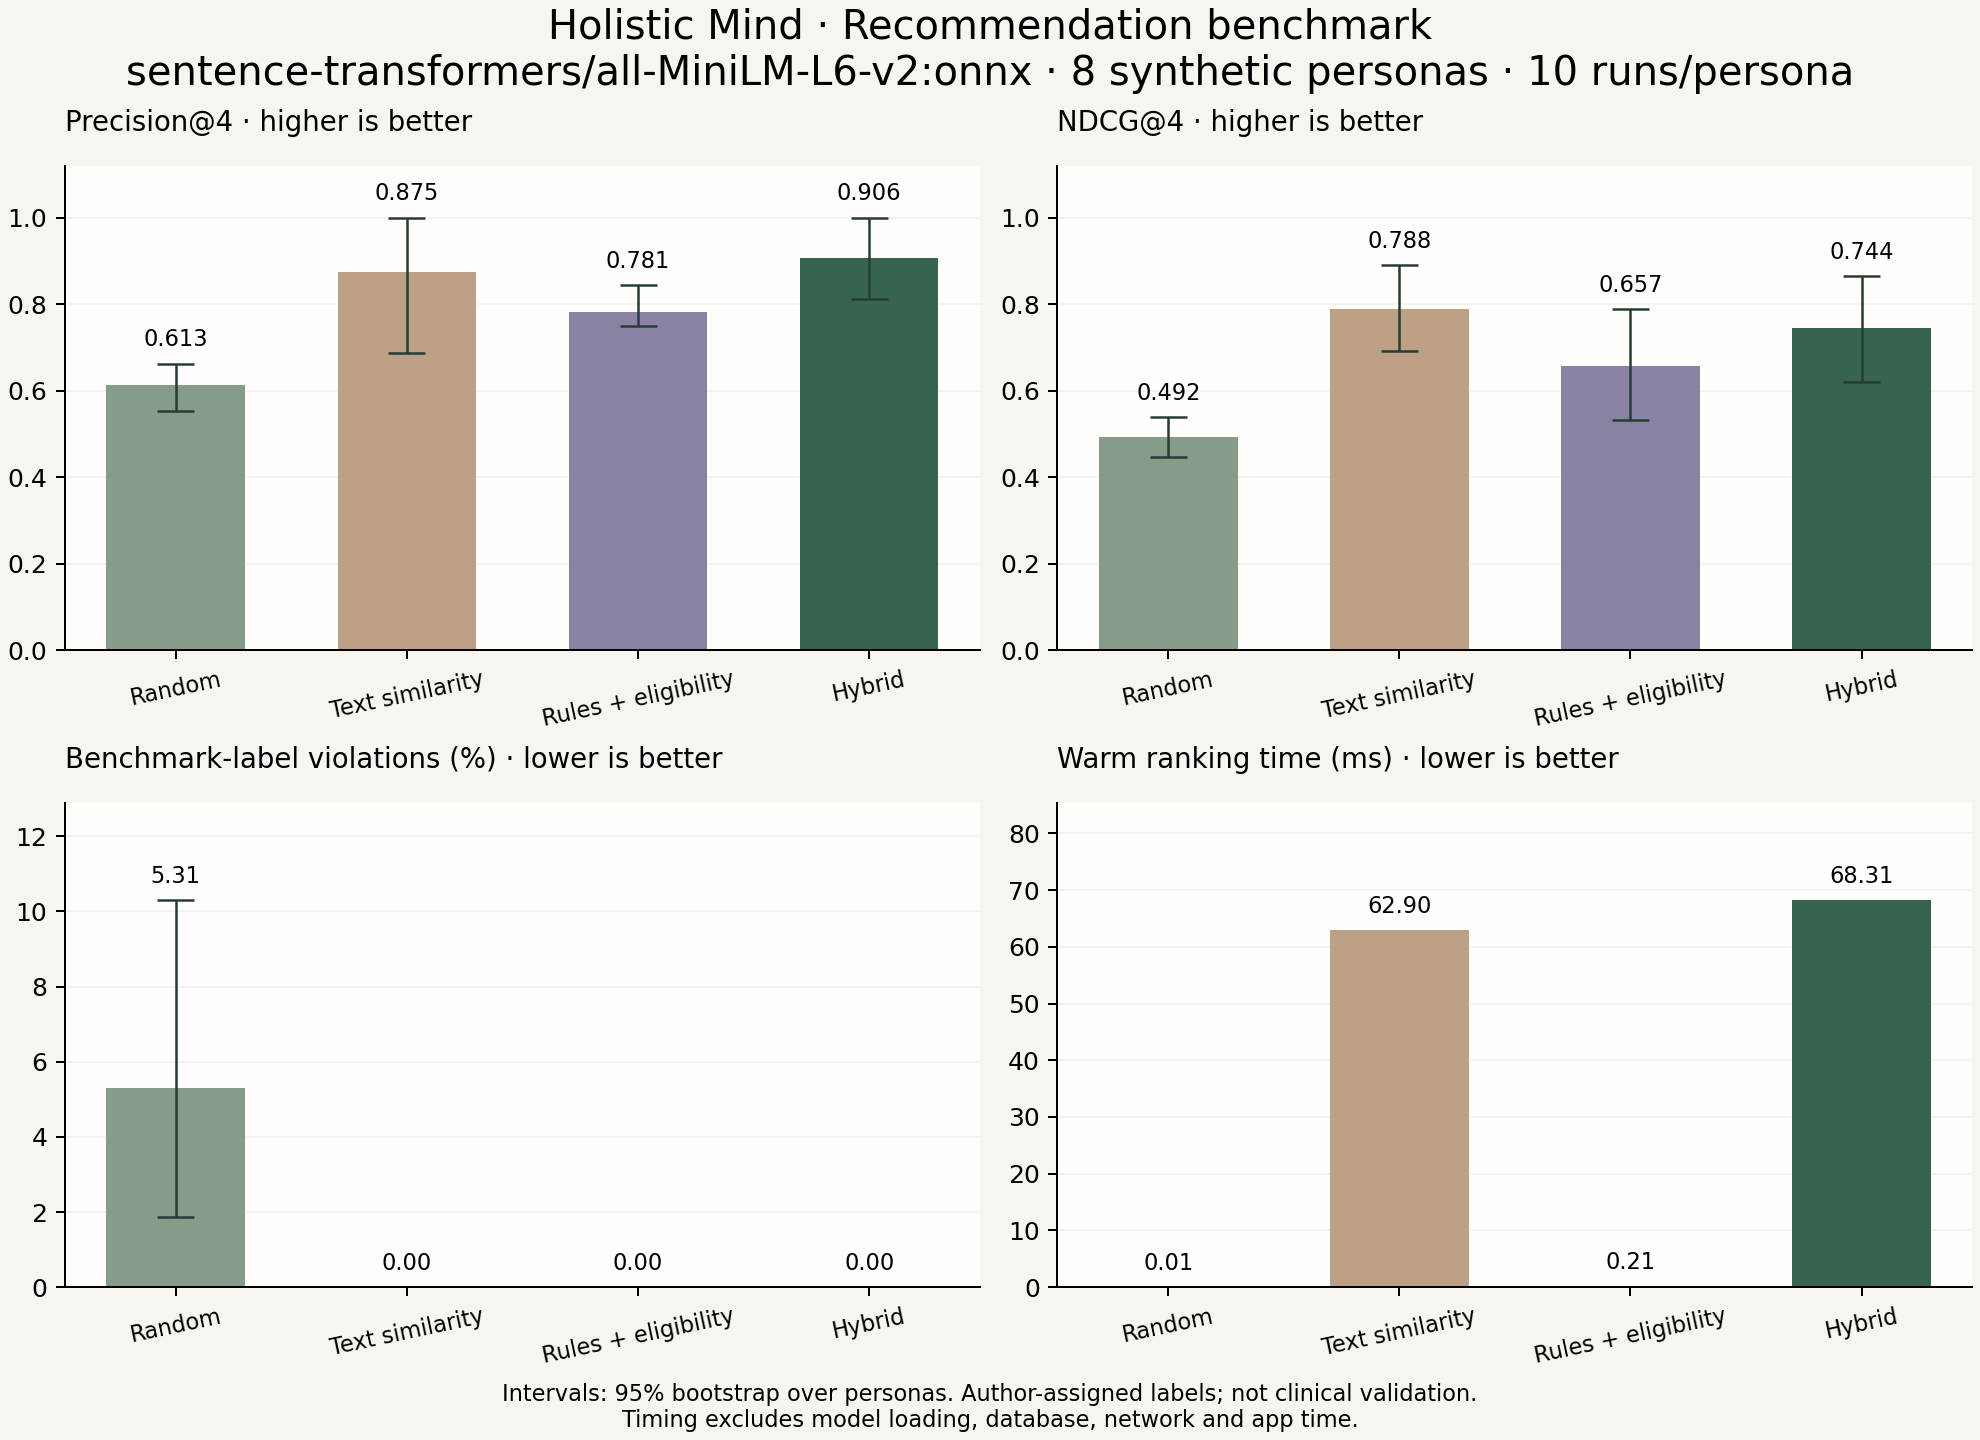
\includegraphics[width=\linewidth,height=0.62\textheight,keepaspectratio]{figures/comfortchart.png}
\caption[Explicit-comfort ONNX benchmark results]{Existing comfort-suite ONNX chart, eight selected scenarios. The suite tests declared restrictions; it does not establish detection of unspoken concerns or representative user performance.}
\label{fig:comfortchart}
\end{figure}
\FloatBarrier

Three original cases remain informative. One describes touch aversion only in synthetic journal text, another describes head or eye scanning discomfort without a corresponding declared choice, and another negatively labels body scanning without a matching metadata restriction. Current production cannot read the journals, and none of these failures should be hidden by inventing preferences after the fact. Separate variants demonstrate that explicit choices trigger exclusions, while the original labels remain unchanged. Independent review is needed for disputed suitability judgments.

\subsection{Documented functional checks}

The September test record reports successful native encryption/\allowbreak{}decryption, Nepali and emoji round trips, recovery-key verification, rejection of different-account decryption, SecureStore readback, and key persistence after terminating and relaunching the application. Live backend checks used temporary synthetic accounts to verify vault setup, encrypted save/\allowbreak{}read, duplicate retry behaviour, account separation, legacy migration, plaintext rejection, comfort-choice persistence, and a live hybrid-v4 ONNX response. Temporary fixtures were cleaned up after those checks.

The same record documents problems with a missing native cryptography module, a simulator build lacking keychain entitlements, and an outdated running recommender container. Rebuilding the native app with the required module and signing, then rebuilding the recommender, resolved those recorded issues. This illustrates why source correctness alone is insufficient for native integration. A library can exist in JavaScript while being absent from the installed binary. Release validation must therefore include the actual installed application and service versions.

\subsection{Metrics, timing, and uncertainty}

Precision and NDCG answer related but different questions. Precision measures the proportion of the requested four slots occupied by exercises with labels of at least two. NDCG rewards stronger labels placed earlier. Recall divides relevant returns by all relevant labelled items for that scenario. MRR concerns the position of the first relevant item. Coverage and category diversity describe catalogue use rather than whether any individual user benefits. Reading these measures together prevents one favourable result from standing in for the complete recommendation experience.

The benchmark's negative-label measure is named safety\_violation\_rate in the saved output, but its meaning is disagreement with authored negative labels. It is not an observed adverse-event rate. Explicit-exclusion violations are a separate property: an exercise can violate an authored label even when the user supplied no corresponding restriction. Conversely, a strongly relevant exercise may be excluded by a user's expressed preference. That is why the comfort suite's unchanged ideal relevance labels can limit interpretation of recall and NDCG.

Timing describes warm, in-process ranking. The saved production chart reports mean times of approximately 0.01 ms for random, 95.24 ms for semantic-only, 0.22 ms for rules, and 79.74 ms for hybrid. The hybrid's lower time than text-only in this run is not proof of universal speed superiority; candidate filtering and measurement variation affect the workload. Model load, tokeniser setup, database queries, HTTP transport, and mobile rendering are excluded. User-perceived delay requires a separate end-to-end measurement.

Bootstrap intervals reflect uncertainty over these authored scenarios. They do not compensate for a biased catalogue, uncertain labels, or a missing held-out dataset. Some comfort cases share a source persona, limiting independence further. The correct conclusion is that the saved runs make technical comparison transparent and reproducible under their recorded conditions. A stronger research claim requires additional data and a design that distinguishes development choices from final evaluation.

\subsection{Verification matrix and regression priorities}

\begingroup
\small\setstretch{1.08}
\setlength{\tabcolsep}{4pt}
\setlength{\TableInnerWidth}{\dimexpr\linewidth-24pt\relax}
\begin{longtable}{@{}>{\raggedright\arraybackslash}p{0.220\TableInnerWidth} >{\raggedright\arraybackslash}p{0.260\TableInnerWidth} >{\raggedright\arraybackslash}p{0.260\TableInnerWidth} >{\raggedright\arraybackslash}p{0.260\TableInnerWidth}@{}}
\caption{Verification evidence by system layer. These are recorded or source-observed results, not newly rerun application tests for this report.}\label{tab:table-4}\\
\toprule
\textbf{Layer} & \textbf{Evidence source} & \textbf{Supported conclusion} & \textbf{Outstanding check} \\
\midrule\endfirsthead
\multicolumn{4}{l}{\textit{Table \thetable\ continued}}\\
\toprule
\textbf{Layer} & \textbf{Evidence source} & \textbf{Supported conclusion} & \textbf{Outstanding check} \\
\midrule\endhead
\midrule\multicolumn{4}{r}{\textit{Continued on next page}}\\\endfoot
\bottomrule\endlastfoot
Mobile types and exports & September/\allowbreak{}October change records & Recorded checks passed & Production-signed device release \\ \addlinespace[4pt]
Comfort policy & Shared mapping; regression suite & Declared exclusions exercised & Usability of preference wording \\ \addlinespace[4pt]
Journal crypto/\allowbreak{}API & Synthetic tests and live API record & Round trips; ownership; migration & Independent security assessment \\ \addlinespace[4pt]
Native key storage & 15 September simulator record & Key persists after restart & Physical-device recovery/\allowbreak{}reinstall \\ \addlinespace[4pt]
Ranking quality & 18 September saved ONNX runs & Authored relevance comparison & Unseen scenarios; expert labels \\ \addlinespace[4pt]
Administration/\allowbreak{}content & Source and September review & Managed publication implemented & Editorial and load validation \\ \addlinespace[4pt]
Provider login & Source and 3 October change record & Configuration and readiness work & Complete current Google login \\ \addlinespace[4pt]
Usability/\allowbreak{}effectiveness & Earlier proposed protocol & Research design available & Consented participant evaluation \\ \addlinespace[4pt]
\end{longtable}
\endgroup

The regression plan should focus on failures with consequences across layers. A declared exclusion should survive backend mapping, Python filtering, diversity selection, and local fallback. An account change should clear the active journal session. A repeated encrypted save should not create duplicate entries. A migration retry should not overwrite an already encrypted record. Recommendation feedback should reject references that do not belong to an owned returned request. These checks test requirements rather than duplicating implementation details.

More recent features require particular care when interpreting older results. The September native record concerns the tested journal modules and synthetic fixtures at that time. It cannot automatically validate later attachment composition or reorganised security screens. The October build/\allowbreak{}export and journal-test record adds evidence for recent changes, but still identifies hands-on recovery UI and physical-device Google sign-in as pending. A versioned verification matrix makes these differences visible to a reviewer.

\subsection{Planned user acceptance evaluation}

The original minimum-five-participant study remains a useful formative proposal. Participants would complete representative tasks, give practice-relevance ratings, and discuss perceived control and confusion. Standard SUS scoring can be used if the instrument is administered without changing its measurement assumptions; an adapted questionnaire should be reported as adapted rather than presented as a standard SUS score. A small study would identify issues and guide iteration, not establish population effectiveness.

A random comparator requires additional care because the software's purpose includes restrictions. A fair user-study comparator should randomise within the same eligible, independently reviewed pool rather than deliberately offer excluded practices. The current offline baseline's omission of suitability rules is acceptable as a clearly documented diagnostic comparison, but does not justify presenting inappropriate content to participants. Appendix C specifies how a future protocol could separate relevance, comfort, task completion, and optional qualitative feedback.

\clearpage\section{Critical Evaluation, Conclusion, and Future Work}\label{sec:chapter-8}

\subsection{Evaluation against objectives}

The source and recorded checks support O1 through implemented account, onboarding, check-in, and persistence pathways, although complete release testing remains open. O2 is supported by a working rules-and-semantic pipeline, recorded score components, and baseline evaluation. O3 has specific evidence for declared exclusions, including short or empty candidate handling. O4 is supported by implemented device encryption and documented native/\allowbreak{}backend round trips. O5 is supported by the administration and content modules. O6 is partially achieved because technical evaluation exists, while representative usability and independent suitability assessment do not.

The strongest engineering result is consistency across boundaries. Declared comfort concerns become explicit constraints, filtered candidates remain excluded during selection, and encrypted journals do not quietly re-enter server recommendation context. The artefact also supports content administration without requiring every content change to become a mobile code change. These outcomes demonstrate useful integration. They do not prove that all content is appropriate or that every deployment path is equally reliable.

\subsection{Threats to validity}

The benchmark is small and authored within the project, so selection and label bias are plausible. A fixed catalogue limits coverage, and preserved labels may reflect expectations inconsistent with newly declared exclusions. Cold-start scenarios cannot assess long-term collaborative behaviour or rotation quality. Repeating deterministic rankers primarily supports timing; it does not enlarge the independent sample. Rules and text baselines differ in eligibility behaviour, so measured improvements cannot be assigned solely to semantic weighting.

Other evidence boundaries concern environment and time. Simulator validation does not establish physical-device signing, interruption handling, reinstall recovery, or Android behaviour. Historical documentation may lag current source. Warm ranking latency excludes network and interface delay. Cryptographic implementation evidence does not replace an independent security review, and current row migration does not erase earlier backups. These limitations should constrain both academic conclusions and public product claims.

\subsection{Usability, maintenance, and practical impact}

The application's practical value lies in reducing the steps between noticing a state and finding an available activity. That value remains plausible rather than measured. A user study should examine whether check-in questions are understandable, whether comfort choices accurately describe what people wish to avoid, and whether recommendation reasons help users make decisions. It should also observe skipped questions and declined practices, because these behaviours may reveal friction that a favourable satisfaction score alone would miss.

Maintenance is equally relevant to future impact. A published exercise can change wording, media, or metadata without changing the ranking code. Such updates may alter semantic similarity or eligibility, making catalogue versioning and regression checks valuable. Journal envelope versions and native cryptography dependencies also require coordinated compatibility. The project should retain reproducible evaluation snapshots while documenting when their catalogue or engine no longer matches a release. This would improve the usefulness of both favourable and unfavourable historical results.

\subsection{Comparison with the reviewed knowledge base}

The artefact applies the combination principle described by \citet{burke2002} through an eligibility gate and a conditional weighted ranker. Its contribution lies in the integration of those mechanisms with a daily mobile workflow, rather than a new general-purpose recommendation algorithm. It uses the pretrained semantic representation described by \citet{reimers2019}, without claiming domain-specific model training. The saved comparison shows a 4.17 percentage-point Precision@4 improvement over rules, but that improvement accompanies a higher negative-label selection rate and does not establish a better experience for users.

The NarraGive work described by \citet{slade2024} motivates attention to several evaluation dimensions rather than a single accuracy score. Holistic Mind reports relevance, ordering, violations, coverage, diversity, and timing. However, its authored, interaction-free fixtures provide a narrower evidence base than an evaluation of actual narrative use. The project's collaborative component exists in implementation but remains untested by the saved cold-start benchmark. Independent access through Explore provides a useful design route outside personalised ranking, although its effect on feedback bias has not been measured.

The mixed evidence reviewed by \citet{matthews2025} also limits interpretation: personalisation does not automatically imply additional mental-health benefit. Holistic Mind demonstrates implemented selection support and a privacy boundary, not a proven therapeutic intervention. Relative to a recommender-platform approach such as \citet{tapuria2024}, it concentrates on selection within a managed exercise catalogue and connects that selection to practice feedback and encrypted reflection. These comparisons identify the artefact's scope and unresolved questions without claiming superiority over systems evaluated on different tasks.

\subsection{Answers to research questions}

RQ1 is answered provisionally: on the journal-free authored benchmark, hybrid ranking improved precision and NDCG over the included alternatives, but also returned more negative-labelled items than rules or semantic-only ranking. RQ2 is supported for declared restrictions by the comfort suite and targeted regression cases; undeclared restrictions remain unresolved. RQ3 is supported at implementation level: encrypted journals persist through the API while the current recommendation route sends no journal text. The resulting loss of reflective context is an intentional design trade-off rather than a missing server decryption feature.

\subsection{Future research and privacy work}

The next priority is independent review of exercise metadata and relevance labels, followed by weight selection on development scenarios and evaluation on unseen cases. A longitudinal dataset should assess feedback adaptation, collaborative activation, and repeated recommendation quality. Physical iOS and Android tests should cover interruptions, secure-storage behaviour, recovery on another device, media, and account deletion. A consented usability study should measure task completion and perceived control, while separate accessibility checks examine contrast, assistive technology, and text scaling.

Further privacy work should examine key rotation, compromised recovery material, background locking, and retention of legacy backups. Any journal-aware personalisation should begin with a distinct local-processing design and its own performance and privacy evaluation. Holistic Mind demonstrates that an integrated wellness application can combine a practical daily workflow, constrained recommendation logic, and device-side journal privacy. Its saved results justify continued development, while the reported violations and evidence gaps identify exactly where stronger validation is still required.

\subsection{Reflection on development decisions}

The strongest continuity across the earlier submissions is the commitment to a supportive, non-diagnostic interaction. The June review's concern about sensitive onboarding shaped later choices to collect short structured answers rather than a personal trauma narrative. Its question about explainable recommendations is addressed through returned reasons and score components. Its question about evaluation beyond random suggestions is addressed through four baseline approaches. The final system therefore develops several early research questions into concrete mechanisms and evidence.

Replacing Firebase was the most substantial architectural change reported in the final progress review. It introduced redevelopment of authentication, data access, and administration, but enabled direct control over relational records and recommendation coordination. The decision is defensible for the resulting artefact, although the supplied material does not document a formal total-cost or security comparison with Firebase. The report should explain the observed benefits without treating a custom backend as inherently superior. Greater control also transfers operational and security responsibilities to the project.

The journal redesign illustrates a second important learning point. An apparently useful recommendation input can conflict with the product's privacy intention. Removing journal context reduced the available semantic evidence and slightly lowered saved NDCG compared with the historical benchmark. The project addressed that trade-off by publishing a journal-free evaluation instead of continuing to promote scores from an input path the app no longer uses. This is stronger research practice than retaining a favourable but mismatched historical result.

Native debugging also changed the understanding of completion. The required module and keychain signing problems showed that an exported JavaScript bundle is not equivalent to a working installed app. The stale recommender container showed that source version and running version can diverge. The October sign-in issue showed that provider configuration is insufficient when the application server is stopped. Each problem crossed a boundary between software layers, supporting the final review's emphasis on systems thinking and maintainability.

\subsection{Practical impact and commercial scope}

The original proposal's freemium idea describes one possible business model, but the current academic contribution does not depend on subscriptions. Introducing paid access would require payment and entitlement handling, clear content boundaries, and a decision about which practices remain available without charge. It would also introduce new usability and retention questions. None of those questions is resolved by the existing recommendation metrics. The report therefore treats monetisation as optional future product work.

Potential impact is concentrated in a coherent routine, clearer content selection, and greater control over reflective privacy. These benefits are plausible from the design but need observation with intended users. A larger library could also create new selection burden if categories and reasons become confusing. More engagement is not automatically better: repeated use might indicate usefulness, habit, distress, or simple curiosity. The project should avoid optimising solely for completion counts and instead assess what users want from the routine.

\subsection{Prioritised completion roadmap}

The first priority is content and metadata review. An independent reviewer should examine descriptions, restrictions, suitability labels, and the three unresolved benchmark cases. The output should be a dated, versioned catalogue and documented label decisions. The second priority is physical-device and release verification, covering provider sign-in, native key storage, recovery on another device, interruptions, attachments, and deletion. These activities close important evidence gaps without introducing a new recommendation feature.

The third priority is a consented formative usability study focused on the complete daily journey and journal setup. It should measure successful task completion, the interpretation of recommendation reasons, and understanding of comfort choices and key-loss consequences. The fourth is ranking research: separate development and unseen scenarios, compare common eligibility policies where appropriate, and evaluate longitudinal feedback and rotation. Only after these foundations are stronger should the project increase collaborative influence or add another personalisation input.

Future journal-aware support should be designed as a separate local-processing capability if pursued. It must not weaken the existing encryption promise by quietly uploading decrypted content or embeddings. Key rotation, recovery-material compromise, background locking, and legacy-backup retention are also concrete privacy priorities. This roadmap preserves the original ambition while directing effort toward validation and control. Holistic Mind's contribution is a functioning, inspectable artefact and a clear account of how its design evolved; its remaining research and release work are identifiable rather than concealed.

\subsection{Conclusion}

Holistic Mind translates an early proposal into an integrated mobile application with an inspectable recommendation pipeline, structured content administration, and device-side journal encryption. The project's development history shows how practical constraints and privacy decisions reshaped the original design. The saved benchmark supports the feasibility of combining rules and semantic similarity, while its negative-labelled selections demonstrate why ranking performance alone is insufficient. The next stage should strengthen content review, device verification, and user acceptance evidence. The report therefore establishes a substantial software contribution and a credible basis for further research without claiming clinical benefit or completed studies that the evidence does not support.

\clearpage\begingroup\setstretch{1.15}\phantomsection\addcontentsline{toc}{section}{References}
\begin{thebibliography}{99}
\bibitem[Burke(2002)]{burke2002}
Burke, R. (2002) 'Hybrid Recommender Systems: Survey and Experiments', User Modeling and User-Adapted Interaction, 12, pp. 331--370. \url{https://doi.org/10.1023/A:1021240730564}.

\bibitem[Fullel(2026)]{fullel2026}
Fullel, S. (2026) Saathi: Nepali Voice Assistant for Elderly Users. Undergraduate project report, Birmingham City University /\allowbreak{} Sunway College Kathmandu. User-supplied PDF; used as a structural reference.

\bibitem[Hevner et al.(2004)]{hevner2004}
Hevner, A. R., March, S. T., Park, J. and Ram, S. (2004) 'Design Science in Information Systems Research', MIS Quarterly, 28(1), pp. 75--105. \url{https://aisel.aisnet.org/misq/vol28/iss1/6/}.

\bibitem[Holistic Mind project(2026a)]{project2026a}
Holistic Mind project (2026a) Current implementation: src/\allowbreak{}, \path{backend/src/}, \path{admin/src/}, and \path{recommender/app/}. Local repository inspected 3 October 2026; implementation evidence, not an independently published source.

\bibitem[Holistic Mind project(2026b)]{project2026b}
Holistic Mind project (2026b) Journal-free evaluation and restriction investigation. \path{recommender/evaluation/PRODUCTION-EVALUATION.md}; \path{evaluation_results_production_onnx.json}; \path{evaluation_results_comfort_onnx.json}. Saved ONNX runs dated 18 September 2026.

\bibitem[Holistic Mind project(2026c)]{project2026c}
Holistic Mind project (2026c) Device and backend test results. \path{samyam docs/DEVICE-AND-BACKEND-TEST-RESULTS.md}. Recorded verification dated 15 September 2026.

\bibitem[Holistic Mind project(2026d)]{project2026d}
Holistic Mind project (2026d) Project development and privacy documentation. \path{samyam docs/15-Week-Development-Journal.md}; \path{samyam docs/journal-privacy.md}; \path{samyam docs/RECOMMENDATION-BENCHMARK.md}. Read alongside current source because some historical sections describe earlier behaviour.

\bibitem[Holistic Mind project(2026e)]{project2026e}
Holistic Mind project (2026e) Recent changes and current recommendation implementation. \path{samyam docs/RECENT-CHANGES.md}; \path{backend/src/routes/recommendations.ts}; \path{recommender/app/engine.py}; \path{src/screens/home/HomeScreen.tsx}. Source inspected 3 October 2026. See Appendix D and the packaged evidence manifest.

\bibitem[Linardon et al.(2019)]{linardon2019}
Linardon, J., Cuijpers, P., Carlbring, P., Messer, M. and Fuller-Tyszkiewicz, M. (2019) 'The efficacy of app-supported smartphone interventions for mental health problems: a meta-analysis of randomized controlled trials', World Psychiatry, 18(3), pp. 325--336. \url{https://pmc.ncbi.nlm.nih.gov/articles/PMC6732686/}.

\bibitem[Matthews and Rhodes-Maquire(2025)]{matthews2025}
Matthews, P. and Rhodes-Maquire, C. (2025) 'Personalisation and Recommendation for Mental Health Apps: A Scoping Review', Behaviour \& Information Technology, 44(10), pp. 2389--2404. \url{https://doi.org/10.1080/0144929X.2024.2356630}.

\bibitem[Morris et al.(2023)]{morris2023}
Morris, J. X., Kuleshov, V., Shmatikov, V. and Rush, A. M. (2023) 'Text Embeddings Reveal (Almost) As Much As Text', Proceedings of EMNLP, pp. 12448--12460. \url{https://aclanthology.org/2023.emnlp-main.765/}.

\bibitem[Rai(2026)]{rai2026}
Rai, A. (2026) A Semantic Approach to Tourist Recommendation in Nepal. Undergraduate dissertation, Birmingham City University. User-supplied PDF; used as a structural reference.

\bibitem[Reimers and Gurevych(2019)]{reimers2019}
Reimers, N. and Gurevych, I. (2019) 'Sentence-BERT: Sentence Embeddings using Siamese BERT-Networks', Proceedings of EMNLP-IJCNLP, pp. 3982--3992. \url{https://aclanthology.org/D19-1410/}.

\bibitem[SAMHSA(n.d.)]{samhsa}
SAMHSA (n.d.) Trauma-Informed Approaches and Programs. \url{https://www.samhsa.gov/mental-health/trauma-violence/trauma-informed-approaches-programs}. Accessed 3 October 2026.

\bibitem[Sentence Transformers(n.d.)]{minilm}
Sentence Transformers (n.d.) all-MiniLM-L6-v2 model card. \url{https://huggingface.co/sentence-transformers/all-MiniLM-L6-v2}. Accessed 3 October 2026.

\bibitem[Shrestha(2026a)]{shrestha2026a}
Shrestha, S. (2026a) Holistic Mind App: A Trauma-Informed Mental Wellness Mobile Application. Project I proposal. User-supplied PDF: Holistic Mind App by Samyam Shrestha.pdf.

\bibitem[Shrestha(2026b)]{shrestha2026b}
Shrestha, S. (2026b) The Holistic Mind: A Trauma-Informed, AI-Powered Mobile Application for Mental Health Self-Regulation. Project Interim Report, CMP6200/\allowbreak{}DIG6200, 27 April. User-supplied PDF: Sunway Interim Report.pdf.

\bibitem[Shrestha(2026c)]{shrestha2026c}
Shrestha, S. (2026c) The Holistic Mind: Interim Progress Review. CMP6200/\allowbreak{}DIG6200, 14 June; reporting period 27 April--14 June. User-supplied PDFs: Interim Progress Review Samyam Shrestha.pdf and Samyam Shrestha Interim Progress Review (1).pdf; duplicate milestone evidence.

\bibitem[Shrestha(2026d)]{shrestha2026d}
Shrestha, S. (2026d) The Holistic Mind: Final Progress Review. CMP6200/\allowbreak{}DIG6200, 2 September. User-supplied PDF: Sunway Final Progress Review.pdf.

\bibitem[Shrestha(n.d.)]{shresthand}
Shrestha, S. (n.d.) Design and Evaluation of a MongoDB-Based IoT Data Platform with MQTT and Smart Automation for IoThings Home Automation Solutions. CMP6207 Modern Data Stores consultancy report. User-supplied PDF: Samyam Shrestha Modern Data Store.pdf. Separate project; used for technical presentation, not Holistic Mind implementation evidence. The supplied cover does not establish an unambiguous submission year.

\bibitem[Slade et al.(2024)]{slade2024}
Slade, E., Rennick-Egglestone, S., Ng, F., Kotera, Y., Llewellyn-Beardsley, J., Newby, C., Glover, T., Keppens, J. and Slade, M. (2024) 'The Implementation of Recommender Systems for Mental Health Recovery Narratives: Evaluation of Use and Performance', JMIR Mental Health, 11, e45754. \url{https://pmc.ncbi.nlm.nih.gov/articles/PMC11015364/}.

\bibitem[Tapuria et al.(2024)]{tapuria2024}
Tapuria, A., Alexander, J., Marchal, A., Cong, C., Meinert, E., Shankar, R., Ananthakrishnan, A. and Lakey, B. (2024) 'Development of a Mental Health Apps Recommender Platform', Studies in Health Technology and Informatics, 316, pp. 1871--1872. \url{https://doi.org/10.3233/SHTI240796}.
\end{thebibliography}
\endgroup\clearpage\appendix
\clearpage\section{Prior-report traceability}

The previous reports contribute different kinds of evidence. The original proposal establishes the intended audience and initial objectives. The April interim report contributes methodology, scope, risk thinking, and a proposed study. The June review contributes prototype milestones and questions about explainability and evaluation. The September review contributes the broader platform description and historical screenshots. Current repository records provide later privacy, comfort, and simulator refinements. The Modern Data Stores coursework is a separate IoT project; its useful influence here is the discipline of relating data models, architecture, security, and evidence to requirements.

\begingroup
\small\setstretch{1.08}
\setlength{\tabcolsep}{4pt}
\setlength{\TableInnerWidth}{\dimexpr\linewidth-24pt\relax}
\begin{longtable}{@{}>{\raggedright\arraybackslash}p{0.240\TableInnerWidth} >{\raggedright\arraybackslash}p{0.290\TableInnerWidth} >{\raggedright\arraybackslash}p{0.240\TableInnerWidth} >{\raggedright\arraybackslash}p{0.230\TableInnerWidth}@{}}
\caption{Source-to-report traceability. Duplicate June progress submissions describe the same reported milestone.}\label{tab:table-5}\\
\toprule
\textbf{Supplied source} & \textbf{Material retained} & \textbf{Final-report location} & \textbf{Qualification} \\
\midrule\endfirsthead
\multicolumn{4}{l}{\textit{Table \thetable\ continued}}\\
\toprule
\textbf{Supplied source} & \textbf{Material retained} & \textbf{Final-report location} & \textbf{Qualification} \\
\midrule\endhead
\midrule\multicolumn{4}{r}{\textit{Continued on next page}}\\\endfoot
\bottomrule\endlastfoot
Holistic Mind App proposal & Audience, motivation, initial objectives & Sections 1 and 3 & Targets distinguished from outcomes \\ \addlinespace[4pt]
Sunway Interim Report & DSR, ethics, scope, study plan & Sections 2--4; Appendix C & Sources checked; study not claimed complete \\ \addlinespace[4pt]
Interim Progress Review & React Native and Firebase prototype & Sections 1, 6, and 8 & Historical stage \\ \addlinespace[4pt]
Interim Progress Review (1) & Same June milestones and questions & Same evidence record & Not a second independent observation \\ \addlinespace[4pt]
Sunway Final Progress Review & Custom services, admin, media, reflection & Sections 5--8; historical Home/\allowbreak{}Explore and Profile/\allowbreak{}History figures & Dated historical implementation \\ \addlinespace[4pt]
Modern Data Store coursework & Clear technical rationale and evidence style & Data and testing presentation & IoT features/\allowbreak{}results not transferred \\ \addlinespace[4pt]
\end{longtable}
\endgroup

Several statements required reconciliation. The initial five-state check-in evolved into six structured dimensions. Firebase was replaced by custom account and data services. The original commercial model did not become evidenced payment infrastructure. The original journal-exclusion intention was temporarily weakened by a journal-context implementation and later strengthened through device encryption and journal-free requests. The final progress review's deployed beta preceded locally verified encryption refinements. These distinctions are retained to make the development account consistent.

Figures~\ref{fig:welcome} and \ref{fig:library} are existing October simulator images. Figures~\ref{fig:home_explore} and \ref{fig:history_profile} reproduce interface evidence from the supplied September review, with the visible account email obscured in Figure~\ref{fig:history_profile}. The remaining explanatory figures were prepared from source and documented decisions; benchmark charts reproduce saved evaluation artefacts. Historical screenshots are labelled by version/\allowbreak{}date and do not establish current physical-device acceptance. Originality declarations and acknowledgements from reference dissertations are not copied into this report.

\clearpage\section{Reproduction and evidence checklist}

A reviewer can begin with the application package scripts and the evaluation README. The production benchmark command is npm run benchmark:production, while npm run benchmark:comfort generates the separate restriction suite. The original journal-containing suite is retained for historical comparison. Strict ONNX mode must successfully load the configured model; a lexical run should remain separately labelled. Output files record engine version, backend identity, catalogue/\allowbreak{}scenario inputs, environment, seed, and source hashes. Repeating a command may overwrite that suite's standard output, so a custom output path should be used when preserving a saved result matters.

The relevant implementation paths are \path{recommender/app/engine.py} and schemas.py; \path{backend/src/routes/recommendations.ts} and \path{data/comfortPreferences.ts}; \path{src/services/recommendations/}; \path{src/services/journal/}; \path{src/context/JournalContext.tsx}; and \path{backend/src/routes/journal.ts}. Database definitions are in \path{backend/src/db.ts}. These are repository-relative paths and can change as the project evolves. Their inclusion provides a starting point for review rather than embedding source code or secrets into the dissertation.

The regression commands include npm run test:comfort, npm run test:journal, npm run recommender:test, and npm run recommender:typecheck. Mobile TypeScript, backend build, and web/\allowbreak{}native bundle exports check different integration boundaries. Journal API tests use synthetic fixtures and isolated database tooling; live native/\allowbreak{}backend tests require the intended services and installed app. A reviewer should record the date, source version, environment, commands, and results of any rerun. The saved passes cited in this report are attributed to their existing records rather than represented as new results.

The release checklist should verify the installed native version, API readiness, database migration status, recommendation model/\allowbreak{}version, storage policy, email delivery, provider client configuration, and journal recovery on an additional device. It should then exercise check-in, restriction enforcement, practice playback, encrypted reflection, attachment saving, history, logout, and deletion using synthetic accounts. Each item should have a recorded outcome and any limitation. No existing user's reflection should be used as an integration fixture.

\clearpage\section{Proposed formative user-study protocol}

This appendix develops the study proposed in the April interim report. It is a prospective protocol, not a completed study or an ethics approval. Recruitment should begin only after the institution's required review and after exercise content is suitable for the tasks. A minimum of five adult participants may support formative usability observations, but cannot provide representative clinical-effectiveness evidence. Participation should not require disclosure of a traumatic history or a diagnosis; any self-identification criteria require clear consent and data minimisation.

Participants would receive a plain-language explanation of purpose, activities, voluntary withdrawal, data handling, and the application's limits. Tasks would use synthetic account data and optional non-sensitive check-in choices. The facilitator would explain how to pause or stop, and participants could skip any practice. No recovery key from a participant's real journal should be collected. A demonstration vault or synthetic entry can be used to assess comprehension of setup and recovery without exposing personal reflections.

The task sequence would cover onboarding, completing a check-in, selecting a comfort preference, reading a recommendation reason, browsing an alternative practice, opening a learning resource, saving a synthetic reflection, locking the journal, and finding history or account controls. Observations would record completion, errors, requests for help, navigation confusion, and understanding of restrictions. Relevance ratings would be collected separately from comfort and perceived usefulness, so a relevant-looking suggestion is not automatically coded as beneficial.

A comparator, if included, should use the same eligible and reviewed content pool and differ only in selection method. Counterbalanced order can reduce simple learning effects, but the small study still remains formative. The study should not reproduce the offline random baseline's missing suitability rules in participant-facing tasks. Any accidental restriction violation should be recorded and investigated rather than hidden in an average relevance score.

A standard usability instrument can supplement task observations, provided its wording and scoring are reported accurately. Interviews should ask what participants expected, which explanations were useful, where control felt insufficient, and what made journal recovery confusing. Analysis can combine task counts with descriptive scores and transparent thematic summaries. In a small sample, individual difficulties are informative; a single aggregate satisfaction score should not conceal them. No clinical symptom-improvement claim follows from a short task session.

The final study report should state recruitment method, participant count, task protocol, consent and withdrawal handling, instrument version, missing responses, and analytic approach. Findings should distinguish observed behaviour from participant opinion and researcher interpretation. Retention should follow the approved research arrangement. Completing this protocol would address the original study objective and provide evidence for interface iteration, while stronger outcome claims would still require a separate research design.

\clearpage\section{Current recommendation implementation evidence}
\label{sec:code-evidence}

This appendix identifies the source used to ground the five-stage explanation. It records inspection rather than a new runtime test. Source hashes in \path{evidence/source-manifest.json} distinguish this snapshot from later edits. The supplied benchmark JSON and summary CSV reproduce saved results rather than invented measurements.

\begin{description}[style=nextline,leftmargin=0pt,labelwidth=0pt,labelsep=0pt]
\item[Request construction and ownership]
\path{backend/src/routes/recommendations.ts}: check-in prerequisite, published catalogue, 180-day interaction aggregation, discomfort exclusions, HMAC pseudonyms, empty journals, and transactional persistence.
\item[Explicit comfort policy]
\path{backend/src/data/comfortPreferences.ts}: four comfort choices shared by backend and mobile fallback.
\item[Filtering, embeddings, scoring, and selection]
\path{recommender/app/engine.py}: hard eligibility, six field contributions, normalised ONNX vectors, conditional neighbours, cold/warm blends, recency, category diversity, and final-slot rotation.
\item[Mobile response and degraded operation]
\path{src/screens/home/HomeScreen.tsx} and \path{src/services/recommendations/recommendationEngine.ts}: preserve successful empty lists, map server IDs to displayable cards, and invoke the distinct local ranker on request failure.
\item[Metric definitions]
\path{recommender/evaluation/metrics.py}: relevance threshold, discounted gain, negative-label violations, diversity, and coverage. Performance values in the report come from the saved journal-free and comfort suites, not from the historical journal-containing suite.
\end{description}

The figures identify their evidence type: screenshots are dated interface records, architecture and workflow diagrams are source-based explanations, and quantitative charts reproduce saved evaluation data. No participant study, current full provider-login acceptance, clinical benefit, or new deployment is inferred from these artefacts.

\end{document}
